\documentclass[aspectratio=169]{beamer}

\usepackage{ctex}
\usepackage{amsmath, amsfonts, amssymb, bm}
\usepackage{graphicx}
\usepackage{hyperref}
\usepackage{booktabs}
\usepackage{array}
\usepackage{tabularx}
\usepackage{ragged2e}
\usepackage{pgfpages}

\usetheme{Berlin}
\usecolortheme{whale}
\useinnertheme[shadow=true]{rounded}
\usefonttheme[onlymath]{serif}
\setbeamercovered{transparent}
\setbeamertemplate{navigation symbols}{}
\setbeamertemplate{bibliography item}[text]
\setbeamercolor{bibliography item}{fg=black}
\setbeamercolor{bibliography entry author}{fg=black}
\setbeamercolor{bibliography entry title}{fg=black}
\setbeamercolor{bibliography entry location}{fg=black}
\setbeamercolor{bibliography entry note}{fg=black}
\hypersetup{hidelinks}

\newcolumntype{Y}{>{\RaggedRight\arraybackslash}X}
\newcommand{\best}[1]{\textbf{#1}}
\newcommand{\mpdata}{relaxed clean equal-atoms MP label}
\newcommand{\hzwdata}{relaxed clean equal-atoms HZW label}
\graphicspath{{figures/story_slides/}{figures/huber_diagnostics/}}
\makeatletter
\newif\ifpympressnotesright
\newif\ifpympressnotesafter
\@ifundefined{pympressnotesright}{\pympressnotesrightfalse}{\pympressnotesrighttrue}
\@ifundefined{pympressnotesafter}{\pympressnotesafterfalse}{\pympressnotesaftertrue}
\makeatother
\ifpympressnotesright
  \setbeameroption{show notes on second screen=right}
\else\ifpympressnotesafter
  \setbeameroption{show notes}
\else
  \setbeameroption{hide notes}
\fi\fi
\newcommand{\speakernote}[1]{\note{\footnotesize #1}}

\setbeamertemplate{footline}{%
 \leavevmode%
 \hbox{%
 \begin{beamercolorbox}[wd=.31\paperwidth,ht=2.25ex,dp=1ex,center]{author in head/foot}
 \insertshortauthor
 \end{beamercolorbox}%
 \begin{beamercolorbox}[wd=.38\paperwidth,ht=2.25ex,dp=1ex,center]{title in head/foot}
 \insertshorttitle
 \end{beamercolorbox}%
 \begin{beamercolorbox}[wd=.31\paperwidth,ht=2.25ex,dp=1ex,center]{date in head/foot}
 \insertshortdate \quad \insertframenumber/\inserttotalframenumber
 \end{beamercolorbox}%
 }
}

\title[论文写作方案]{晶体带隙预测 GNN 项目论文写作方案}
\subtitle{从失败假设、数据审计到可投稿主线}
\author[刘嘉瑞]{汇报人：刘嘉瑞}
\institute[GNN Bandgap]{任务：晶体 band\_gap 回归预测\\主线：Virtual Node / Huber Loss / MP--HZW Label Consistency}
\date{2026年7月}

\begin{document}

\begin{frame}
 \titlepage
\speakernote{这次不是再讲一遍所有实验，而是回答老师的问题：这堆实验怎么组织成一篇论文。开场先说明今天汇报的是论文写作方案，包括论文题目、核心故事线、章节结构、结果取舍和结论边界。}
\end{frame}

\begin{frame}{目录}
 \tableofcontents
\speakernote{目录快速过。重点是先确定论文主张，再确定每一节写什么证据，最后说明哪些实验进正文，哪些只放附录。}
\end{frame}

\section{论文定位}

\begin{frame}{本次 PPT 的目标}
\small
\begin{block}{老师现在关心的问题}
不是“哪个实验跑赢了”，而是：\best{这些实验怎样写成一篇逻辑自洽的论文}。
\end{block}

\begin{block}{本次要交代清楚}
\begin{itemize}
  \item 论文题目和中心论点是什么。
  \item Introduction 怎么从材料问题引到模型问题和数据问题。
  \item Methods / Results / Discussion 分别放哪些内容。
  \item 哪些结论能写进正文，哪些只能作为探索或附录。
\end{itemize}
\end{block}
\speakernote{这里要把汇报目标转过来。老师要的是论文梳理，所以不要陷入每个实验细节，而是讲文章怎么立起来。}
\end{frame}

\begin{frame}{拟定英文题目}
\small
\begin{alertblock}{推荐题目}
\centering
\textbf{Robust Global Virtual-Node Graph Neural Networks for Crystal Band-Gap Prediction with Cross-Source Label Consistency Analysis}
\end{alertblock}

\vspace{2mm}
\begin{itemize}
  \item \textbf{Robust}：对应 Huber loss，是最终跨源稳定收益。
  \item \textbf{Global Virtual-Node}：对应 single plain virtual node，是主模型改进。
  \item \textbf{Band-Gap Prediction}：明确任务边界。
  \item \textbf{Cross-Source Label Consistency}：对应 MP--HZW 标签冲突审计，是论文区别于普通模型堆叠的关键。
\end{itemize}
\speakernote{题目不要只写模型，也要写数据一致性。因为真正把故事讲完整的是模型和数据双主线：模型上有 virtual node 和 Huber，数据上有 MP-HZW 标签冲突审计。}
\end{frame}

\begin{frame}{一句话故事线}
\large
\centering
我们一开始以为问题是 \best{GNN 缺少全局信息}，\\
\vspace{2mm}
后来发现真正稳定的结论是：\\
\vspace{3mm}
\Large
\best{简单全局节点 + 鲁棒损失 + 数据源审计}
\vspace{3mm}

\large
比复杂全局注意力或双槽位更可靠。
\speakernote{这页是全文故事线。注意语气要谨慎，不是否定全局信息，而是把结论从“越复杂越好”修正为“简单全局节点加鲁棒损失最稳”。}
\end{frame}

\begin{frame}{故事线不是“堆实验”，而是“假设被修正”}
\centering
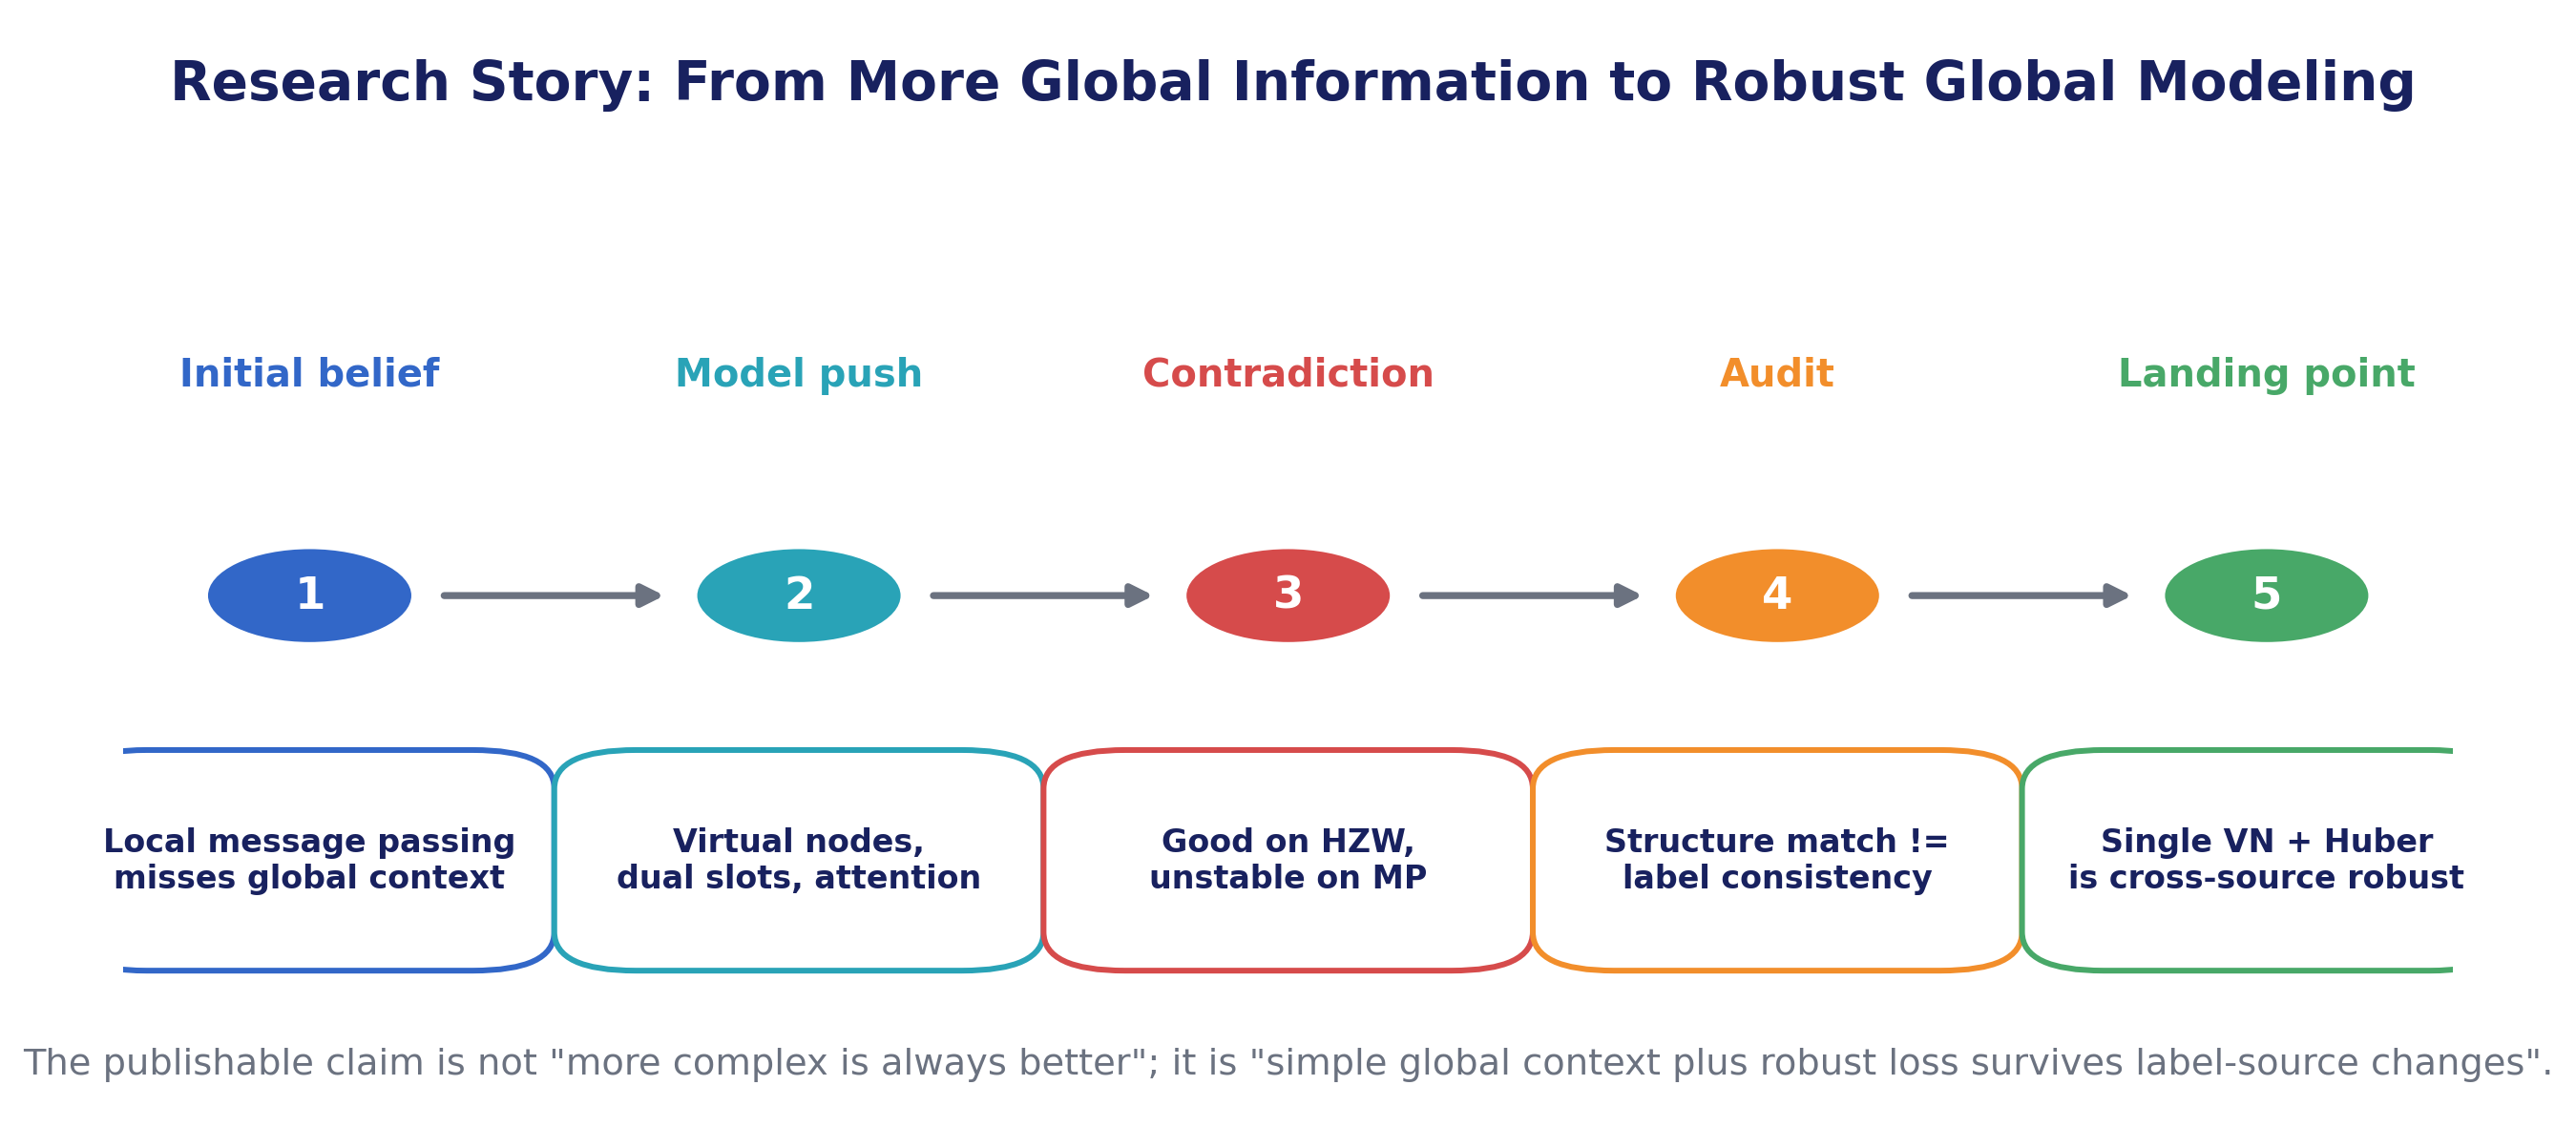
\includegraphics[width=\textwidth,height=0.76\textheight,keepaspectratio]{story_arc.png}
\speakernote{这一页用来替代流水账开场。讲法是：第一步我们怀疑局部消息传递缺少全局上下文；第二步做 virtual node、双槽位、attention；第三步发现跨 MP 和 HZW 不稳定；第四步做数据审计；最后收束到 single VN + Huber。}
\end{frame}

\begin{frame}{这篇论文要回答四个连续问题}
\centering
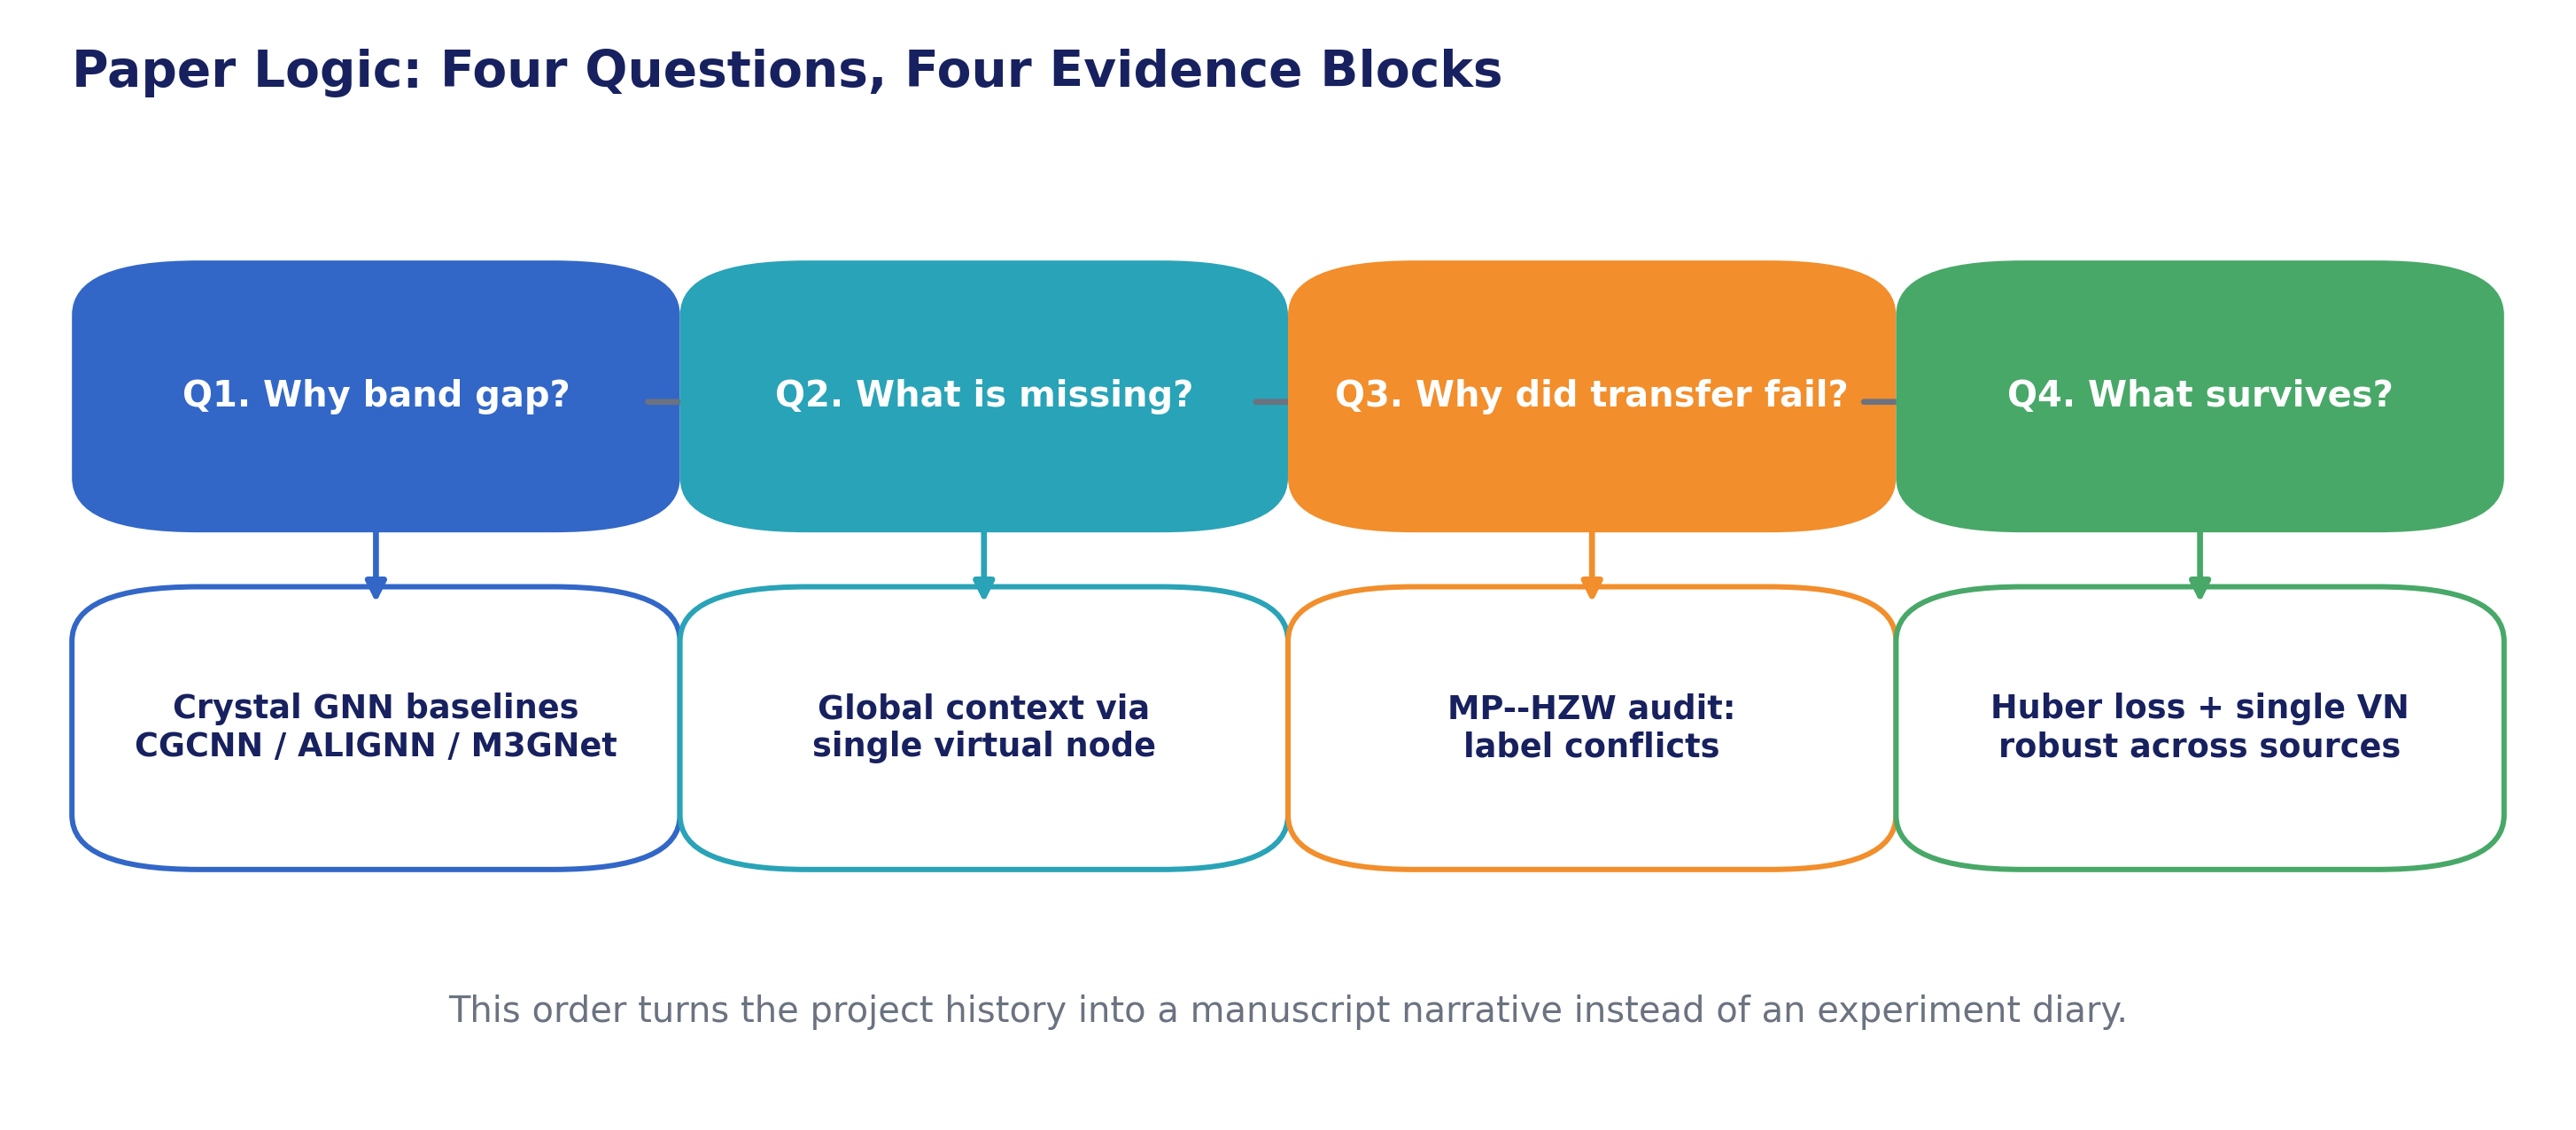
\includegraphics[width=\textwidth,height=0.76\textheight,keepaspectratio]{paper_logic_map.png}
\speakernote{这页把论文结构讲成连续问题，而不是章节清单。先问为什么做 band gap，再问模型缺什么，再问为什么转移失败，最后问什么结论能跨数据源保留下来。}
\end{frame}

\begin{frame}{论文中心论点}
\small
\begin{enumerate}
  \item 晶体 band gap 预测中，ALIGNN 已经建模了关键局部几何；额外全局机制必须小心验证。
  \item Single plain virtual node 是低风险、稳定的全局信息补充。
  \item MP--HZW 结构匹配不等于标签一致；标签冲突会改变模型排序。
  \item Huber loss 是跨 MP label 与 HZW label 最稳定的进一步收益。
  \item Global broadcast decay 只应写成 MP-label-specific improvement，不能写成跨源统一最优。
\end{enumerate}
\speakernote{这一页相当于论文摘要里的核心判断。尤其要强调 T10 不能吹成最终唯一最优，因为 HZW 上 T7 更好。}
\end{frame}

\begin{frame}{论文贡献应该怎么写}
\small
\begin{block}{Contribution 1：模型谱系}
系统比较 CGCNN、ALIGNN、M3GNet 与多种 ALIGNN 全局增强模型，确认 \best{ALIGNN + single plain virtual node} 是稳定强基线。
\end{block}

\begin{block}{Contribution 2：数据审计}
提出 MP--HZW structure-first audit，证明 \best{结构匹配与标签一致性必须分开处理}。
\end{block}

\begin{block}{Contribution 3：最终消融}
在同一批 84,550 结构上分别使用 MP label 和 HZW label 训练，发现 \best{Huber loss 是跨源最稳定收益来源}。
\end{block}
\speakernote{贡献点要控制在三条，不要把每个实验都写成贡献。真正能站住的是模型谱系、数据审计、最终消融。}
\end{frame}

\begin{frame}{哪些话不能写太满}
\small
\begin{tabularx}{\textwidth}{p{4.8cm} Y}
\toprule
不要这么写 & 应该这么写 \\
\midrule
双超节点在所有数据集上有效。 & 双节点在 HZW 早期和大结构分桶上有局部信号，但跨源不稳定。 \\
T10 是最终最强模型。 & T10 是 MP label 最优；跨源最稳是 T7。 \\
MP 和 HZW 是同一数据。 & MP/HZW 可以结构匹配，但 band gap 标签存在冲突。 \\
Top-k 是核心创新。 & Top-k 是信息流探索，独立收益不稳定。 \\
物理约束完整解决问题。 & 物理约束依赖有效 CBM/VBM 标签，适合作为早期探索或附录。 \\
\bottomrule
\end{tabularx}
\speakernote{这页是防止论文被老师或审稿人质疑。我们不夸大复杂模型，只写实验能支撑的结论。}
\end{frame}

\section{文章结构}

\begin{frame}{论文结构总览}
\scriptsize
\centering
\begin{tabularx}{\textwidth}{p{3.0cm} Y p{3.7cm}}
\toprule
章节 & 主要内容 & 需要支撑的图表 \\
\midrule
Abstract & 背景、方法、数据审计、最终结果、结论边界。 & 关键数字：T7/T10 MAE。 \\
Introduction & 从 band gap 任务引出 GNN、全局信息和标签一致性问题。 & 贡献三点。 \\
Related Work & CGCNN、ALIGNN、M3GNet、virtual node、Huber、MP/Matbench。 & 文献表。 \\
Data and Audit & MP--HZW structure-first audit 与 relaxed clean 口径。 & 数据阶段表、冲突计数表。 \\
Methods & Baseline、single VN、Huber、top-k、decay、physics loss。 & 模型公式。 \\
Results & 早期 HZW、MP full、S 系列、最终 T 系列。 & 主结果表。 \\
Discussion & 为什么复杂机制不稳，为什么 decay 只在 MP 有效。 & T7/T10 分析表。 \\
Conclusion & 收敛到 T7 主张，给出局限和后续工作。 & 无需新实验。 \\
\bottomrule
\end{tabularx}
\speakernote{这页给老师看文章骨架。注意 Results 不要按流水账写 E1 到 E13，而是按“早期动机、转折、最终验证”写。}
\end{frame}

\begin{frame}{Abstract 怎么写}
\small
\begin{block}{推荐结构}
\begin{enumerate}
  \item 背景：band gap 是材料发现关键任务，GNN 是重要方法。
  \item 问题：局部消息传递可能缺少全局信息；跨数据源 band gap 标签不一致。
  \item 方法：比较 CGCNN/ALIGNN/M3GNet，提出 single VN、Huber、top-k/decay 消融。
  \item 数据：MP--HZW structure-first audit，最终 84,550 结构双标签源验证。
  \item 结果：MP 最优 T10 = 0.223686，HZW 最优 T7 = 0.194002。
  \item 结论：跨源最稳是 ALIGNN + single VN + Huber。
\end{enumerate}
\end{block}
\speakernote{摘要要一口气讲完模型和数据两条线。不能只写模型，也不能只写数据清洗。}
\end{frame}

\begin{frame}{Introduction 写作逻辑}
\small
\begin{columns}[T,onlytextwidth]
\begin{column}{0.49\textwidth}
\begin{block}{漏斗式展开}
\begin{enumerate}
  \item Band gap 对材料筛选重要。
  \item GNN 可以直接利用晶体结构。
  \item ALIGNN 等局部几何模型已经很强。
  \item 局部消息传递可能缺少全局上下文。
  \item 但是复杂全局机制是否稳定，需要数据源验证。
\end{enumerate}
\end{block}
\end{column}
\begin{column}{0.49\textwidth}
\begin{alertblock}{真正的问题}
问题不只在模型。HZW 和 MP 的结构可以对齐，但 band gap 标签不总是一致；如果不先做数据审计，后面的模型优劣很容易讲错。
\end{alertblock}
\end{column}
\end{columns}
\speakernote{Introduction 要把“全局信息问题”和“标签一致性问题”连起来。这样文章不是普通调参，而是有方法和数据质量两个层次。}
\end{frame}

\begin{frame}{Related Work 怎么组织}
\small
\begin{block}{不要按时间流水账，要按主题}
\begin{itemize}
  \item \textbf{Crystal GNN baselines}：CGCNN、ALIGNN、M3GNet。
  \item \textbf{Global tokens / virtual nodes}：解释为什么需要低成本全局通道。
  \item \textbf{Robust regression}：Huber loss 如何处理重尾误差和标签冲突。
  \item \textbf{Materials datasets}：MP、Matbench，以及跨源标签一致性问题。
\end{itemize}
\end{block}

\begin{block}{写作重点}
Related Work 最后要自然过渡到：本文不是只提出新层，而是把 \best{模型设计、鲁棒损失和数据一致性审计} 放在同一框架下验证。
\end{block}
\speakernote{相关工作不要堆很多模型名。按四个主题写，最后把缺口落到本文自己的贡献上。}
\end{frame}

\begin{frame}{Data and Audit 章节怎么写}
\small
\begin{block}{这一节的主张}
本文的关键数据结论是：\best{structure matched 不等于 label consistent}。
\end{block}

\begin{columns}[T,onlytextwidth]
\begin{column}{0.48\textwidth}
\begin{block}{要写的流程}
\begin{itemize}
  \item HZW 与 MP 记录对齐。
  \item 先判断结构是否匹配。
  \item 在结构匹配样本内统计标签冲突。
  \item 构造 relaxed clean equal-atoms 口径。
\end{itemize}
\end{block}
\end{column}
\begin{column}{0.48\textwidth}
\begin{block}{要放的数字}
\begin{itemize}
  \item 95,462 total rows。
  \item 92,787 structure matched。
  \item 7,984 zero/nonzero conflicts removed。
  \item final accepted 84,550。
\end{itemize}
\end{block}
\end{column}
\end{columns}
\speakernote{数据章节是论文区分度很高的地方。要把清洗讲成审计流程，而不是简单说删了哪些数据。}
\end{frame}

\begin{frame}{数据转折：结构能对上，标签不一定能对上}
\centering
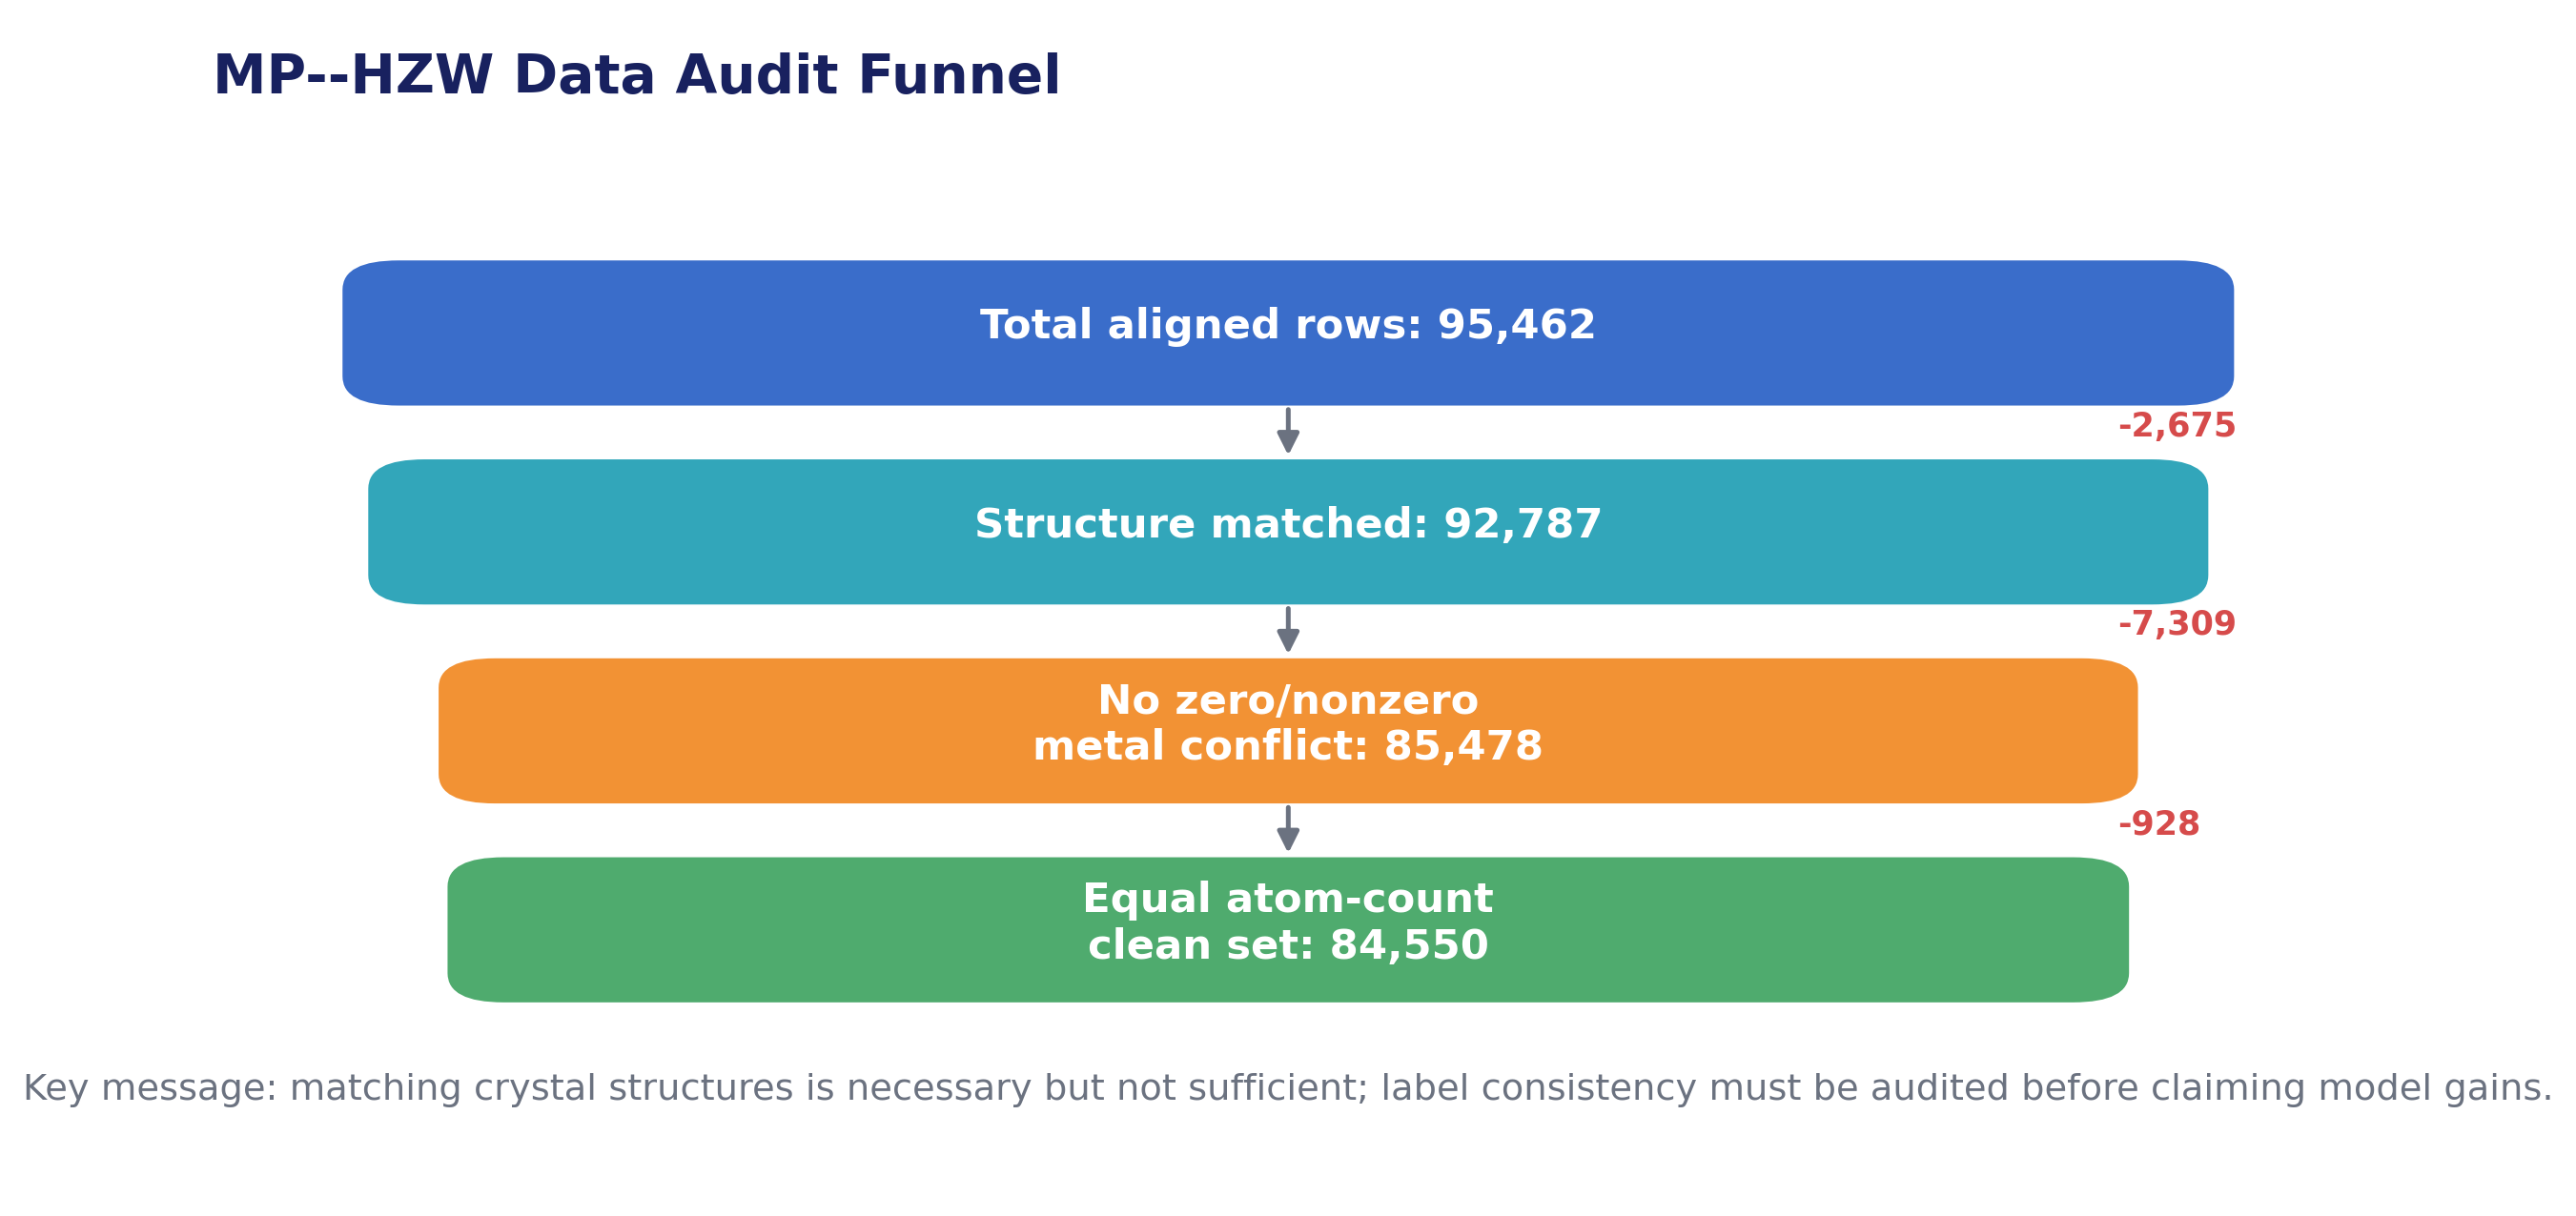
\includegraphics[width=\textwidth,height=0.76\textheight,keepaspectratio]{data_audit_funnel.png}
\speakernote{这页要讲成转折点：如果只说 MP 和 HZW 来自同源，很容易被质疑；我们真正做的是先结构对齐，再看标签冲突。最终 84,550 是用于最终 T 系列的干净 equal-atoms 口径。}
\end{frame}

\begin{frame}{Methods 章节怎么写}
\small
\begin{block}{正文只保留必要方法}
\begin{itemize}
  \item Baselines：CGCNN、ALIGNN、M3GNet，用 1 段说明。
  \item Single plain VN：作为主架构改进，给公式。
  \item Huber loss：作为最终稳定收益，给公式和直觉。
  \item Top-k / warmup / decay：作为 T 系列消融，简洁写。
  \item Physics loss / dual slot：简述早期探索，详细定义放附录。
\end{itemize}
\end{block}

\begin{alertblock}{写作原则}
Methods 不是代码说明书；只写复现实验和理解结果所必需的结构。
\end{alertblock}
\speakernote{方法章节要克制。E14-E19 那些探索如果全塞进正文，主线会散。主文聚焦 single VN、Huber、decay。}
\end{frame}

\begin{frame}{完整架构图：从输入晶体到输出 band gap}
\centering
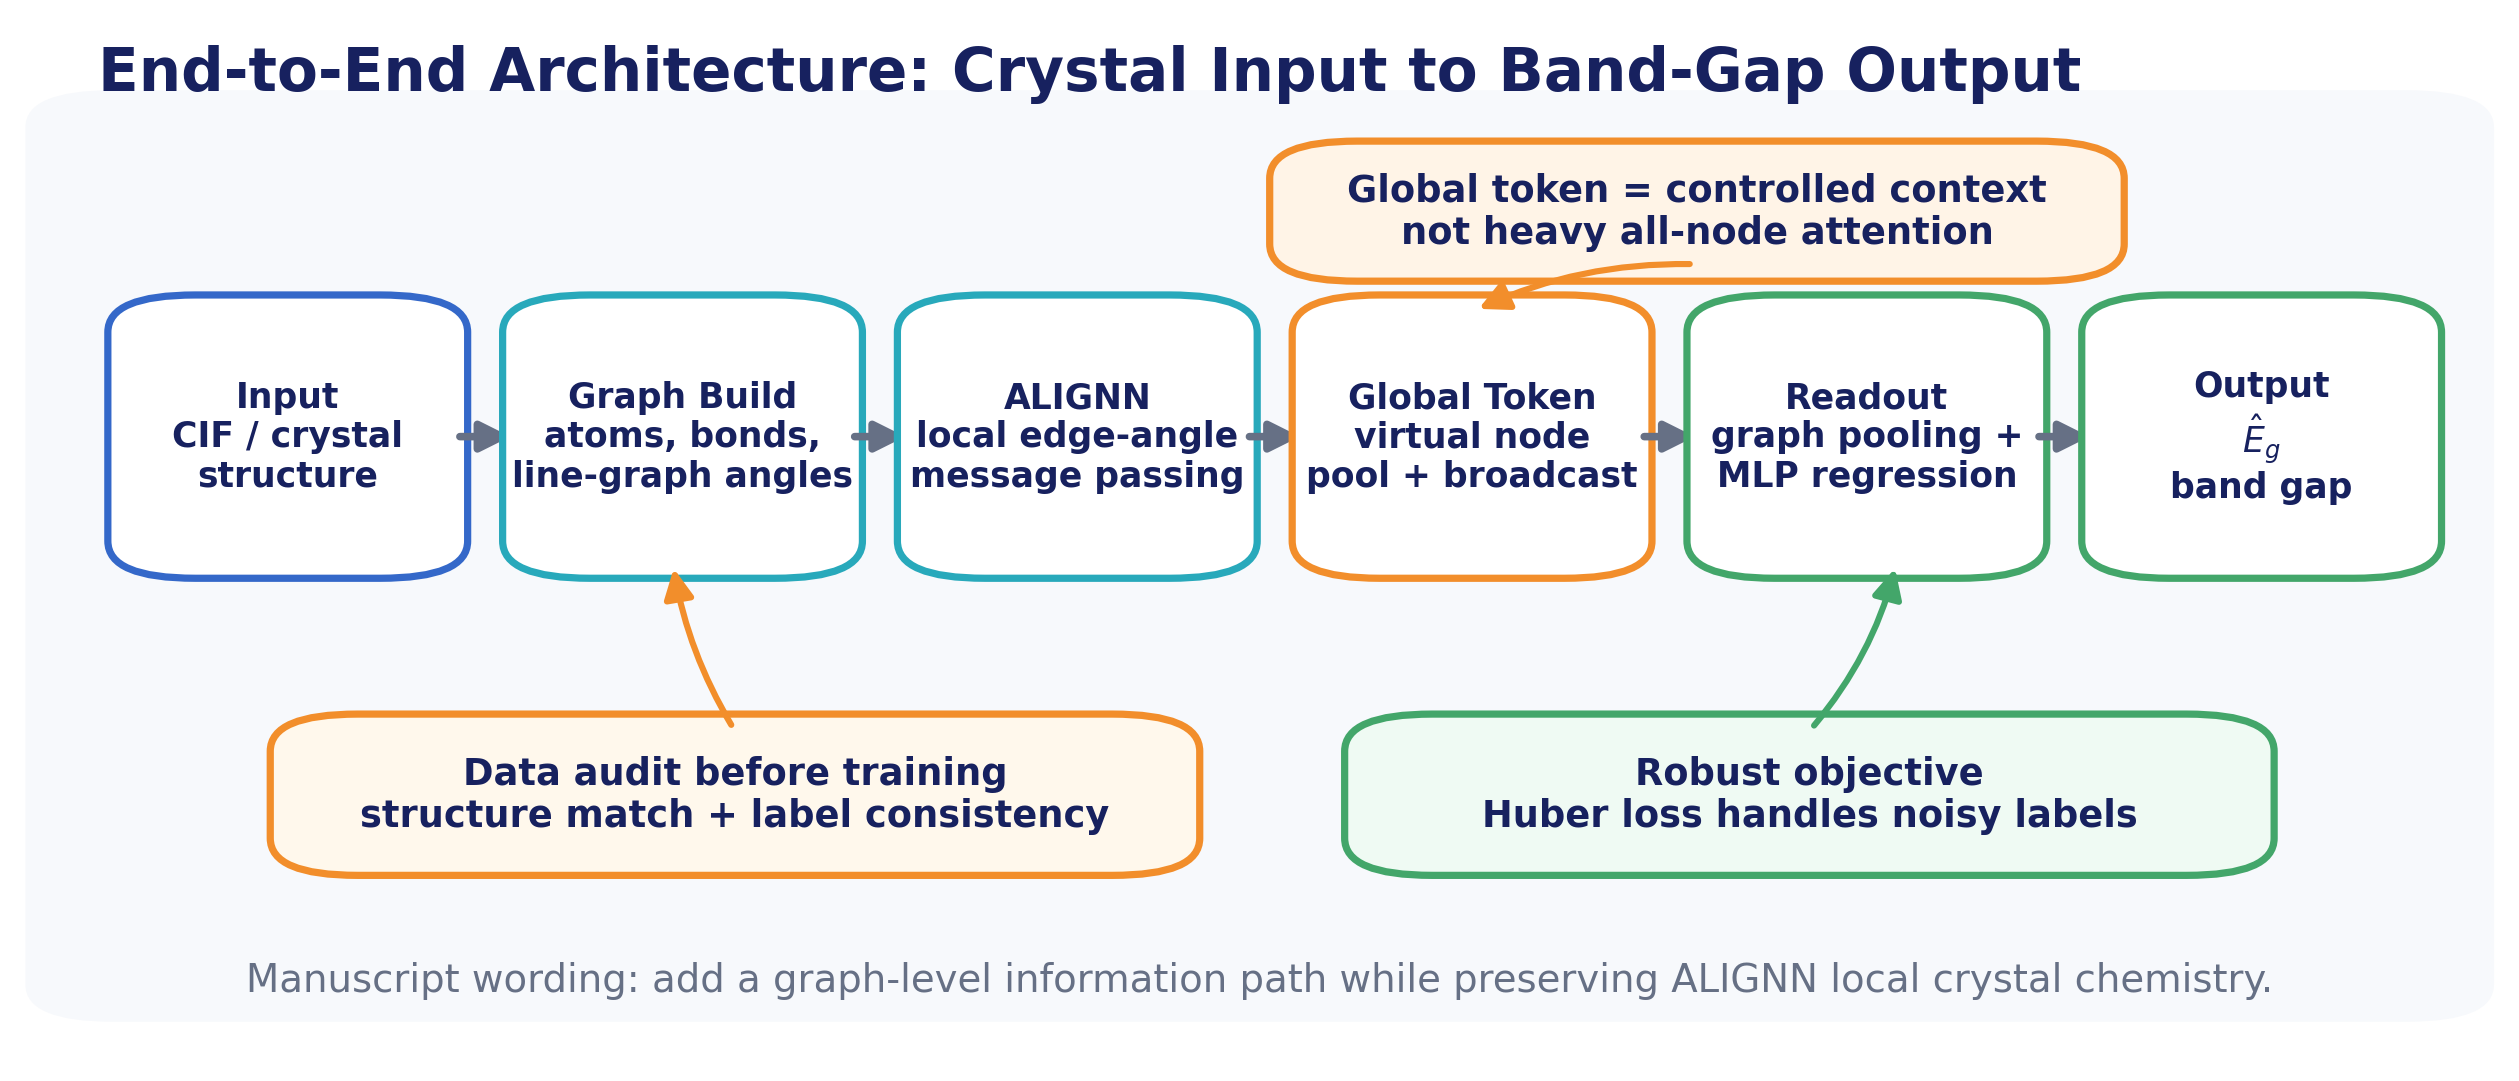
\includegraphics[width=\textwidth,height=0.76\textheight,keepaspectratio]{input_to_output_architecture.png}
\speakernote{这一页回应“缺少从输入到输出架构图”的问题。讲法是：输入是 CIF 或晶体结构；先构建 atom/bond/angle 图；ALIGNN 负责局部边角几何；global token 提供受控全局上下文；最后 graph readout 输出 band gap。数据审计和 Huber loss 是模型外但论文主线内的关键细节。}
\end{frame}

\begin{frame}{主模型图：局部几何先交给 ALIGNN，全局只加低风险通道}
\centering
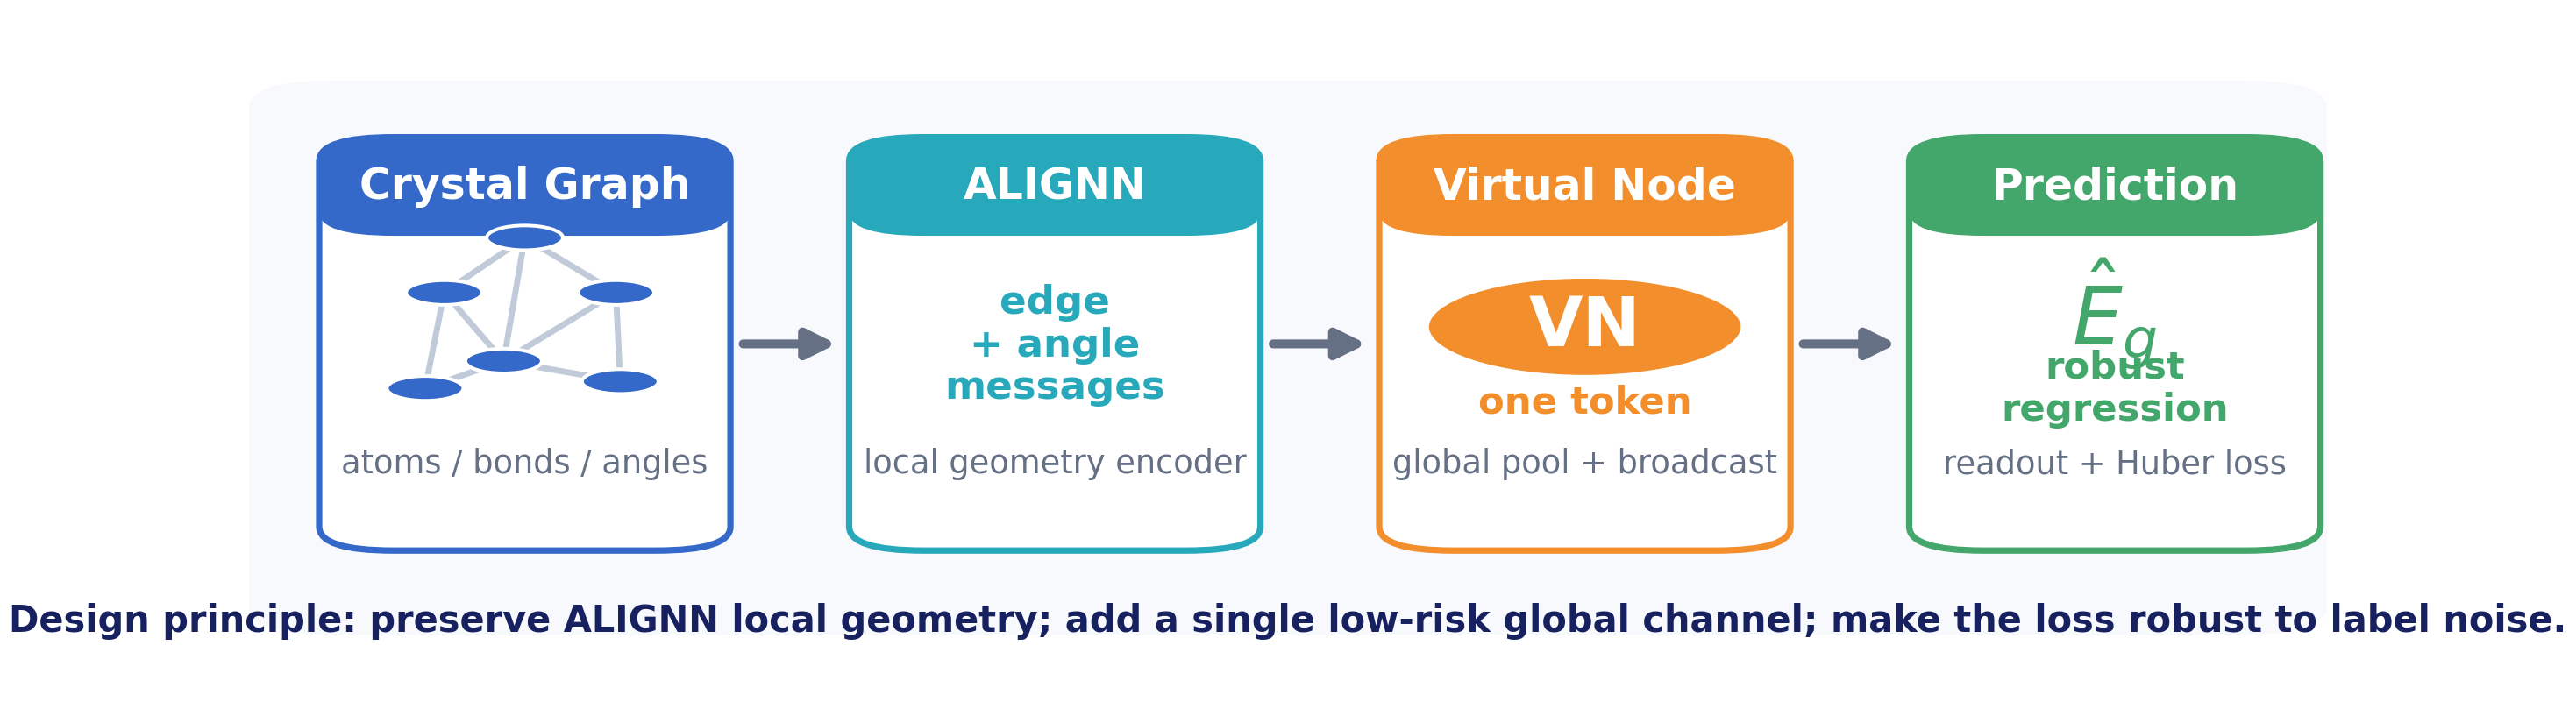
\includegraphics[width=\textwidth,height=0.76\textheight,keepaspectratio]{final_model_architecture.png}
\speakernote{这页要讲清楚为什么最后不吹复杂 attention。ALIGNN 已经编码边和角度，single virtual node 只是增加一个低成本全局汇聚和广播通道，Huber loss 用来抵抗标签冲突和长尾误差。}
\end{frame}

\begin{frame}{Huber loss 的直觉：不是追求更复杂，而是降低脏标签破坏力}
\centering
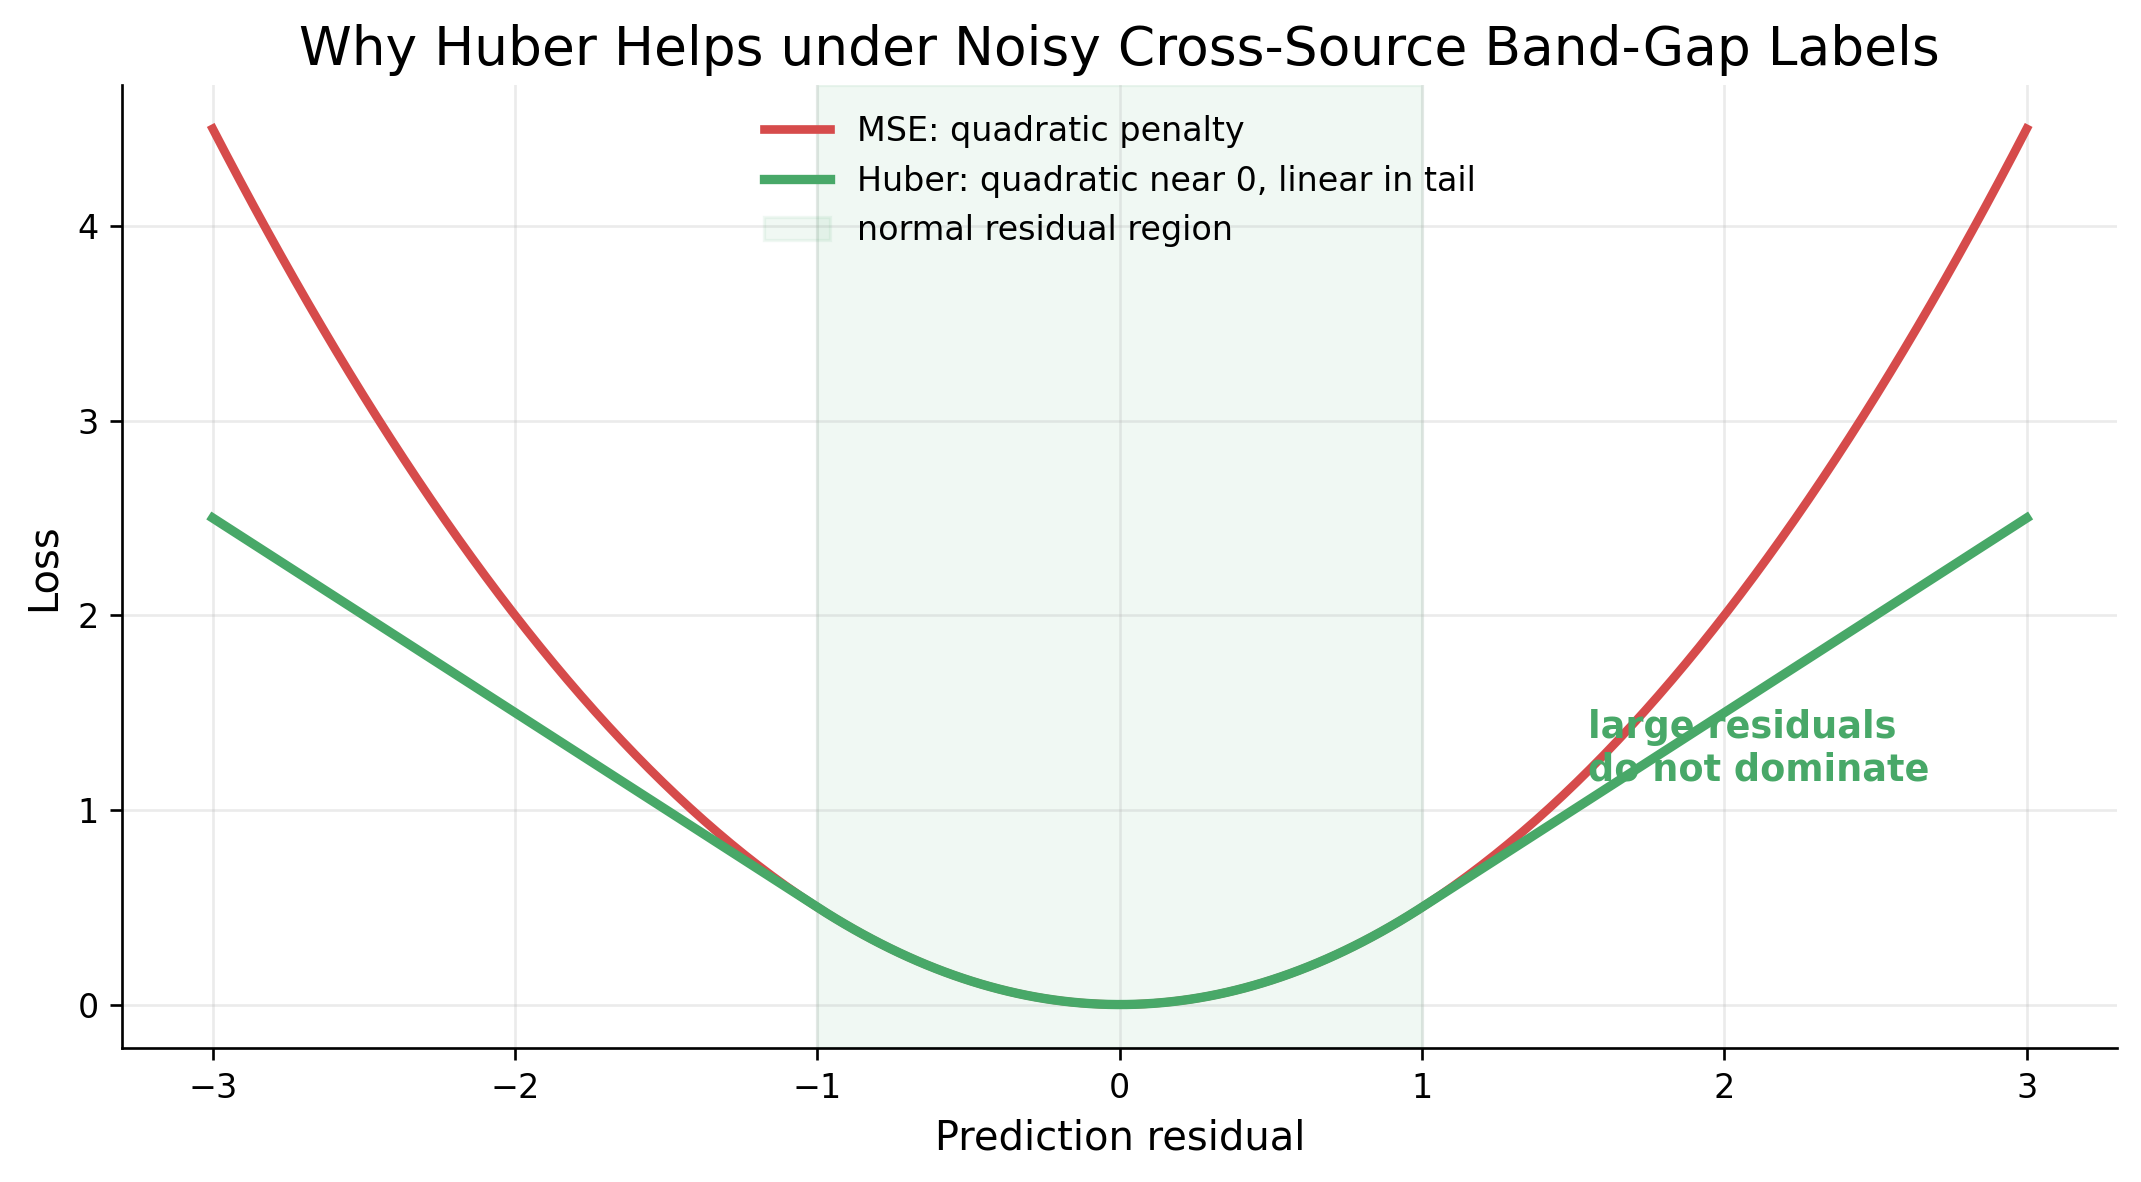
\includegraphics[width=0.86\textwidth,height=0.72\textheight,keepaspectratio]{huber_loss_intuition.png}
\speakernote{这里用直觉讲 Huber。MSE 对大残差平方惩罚，容易被标签冲突或异常样本牵着走；Huber 在残差很大时变成线性惩罚，所以 T7 在 MP 和 HZW 上都稳定。}
\end{frame}

\begin{frame}{Results 章节怎么组织}
\small
\begin{enumerate}
  \item \textbf{Early HZW motivation}：说明为什么开始探索 virtual node、dual slot 和 physics。
  \item \textbf{MP transfer failure}：说明复杂机制不是无条件成立。
  \item \textbf{Data audit}：解释模型排序变化不能只怪模型。
  \item \textbf{Final T-series}：用同一批 84,550 结构，分别看 MP label 和 HZW label。
  \item \textbf{Ablation conclusion}：T4$\rightarrow$T7 是最干净收益，T7$\rightarrow$T10 体现标签源依赖。
\end{enumerate}
\speakernote{Results 要按叙事顺序，不按实验编号。先讲动机，再讲转折，再讲最终验证。这样读者会理解为什么有这么多实验。}
\end{frame}

\begin{frame}{最终证据先看图：T7 跨源稳，T10 是 MP 特化}
\centering
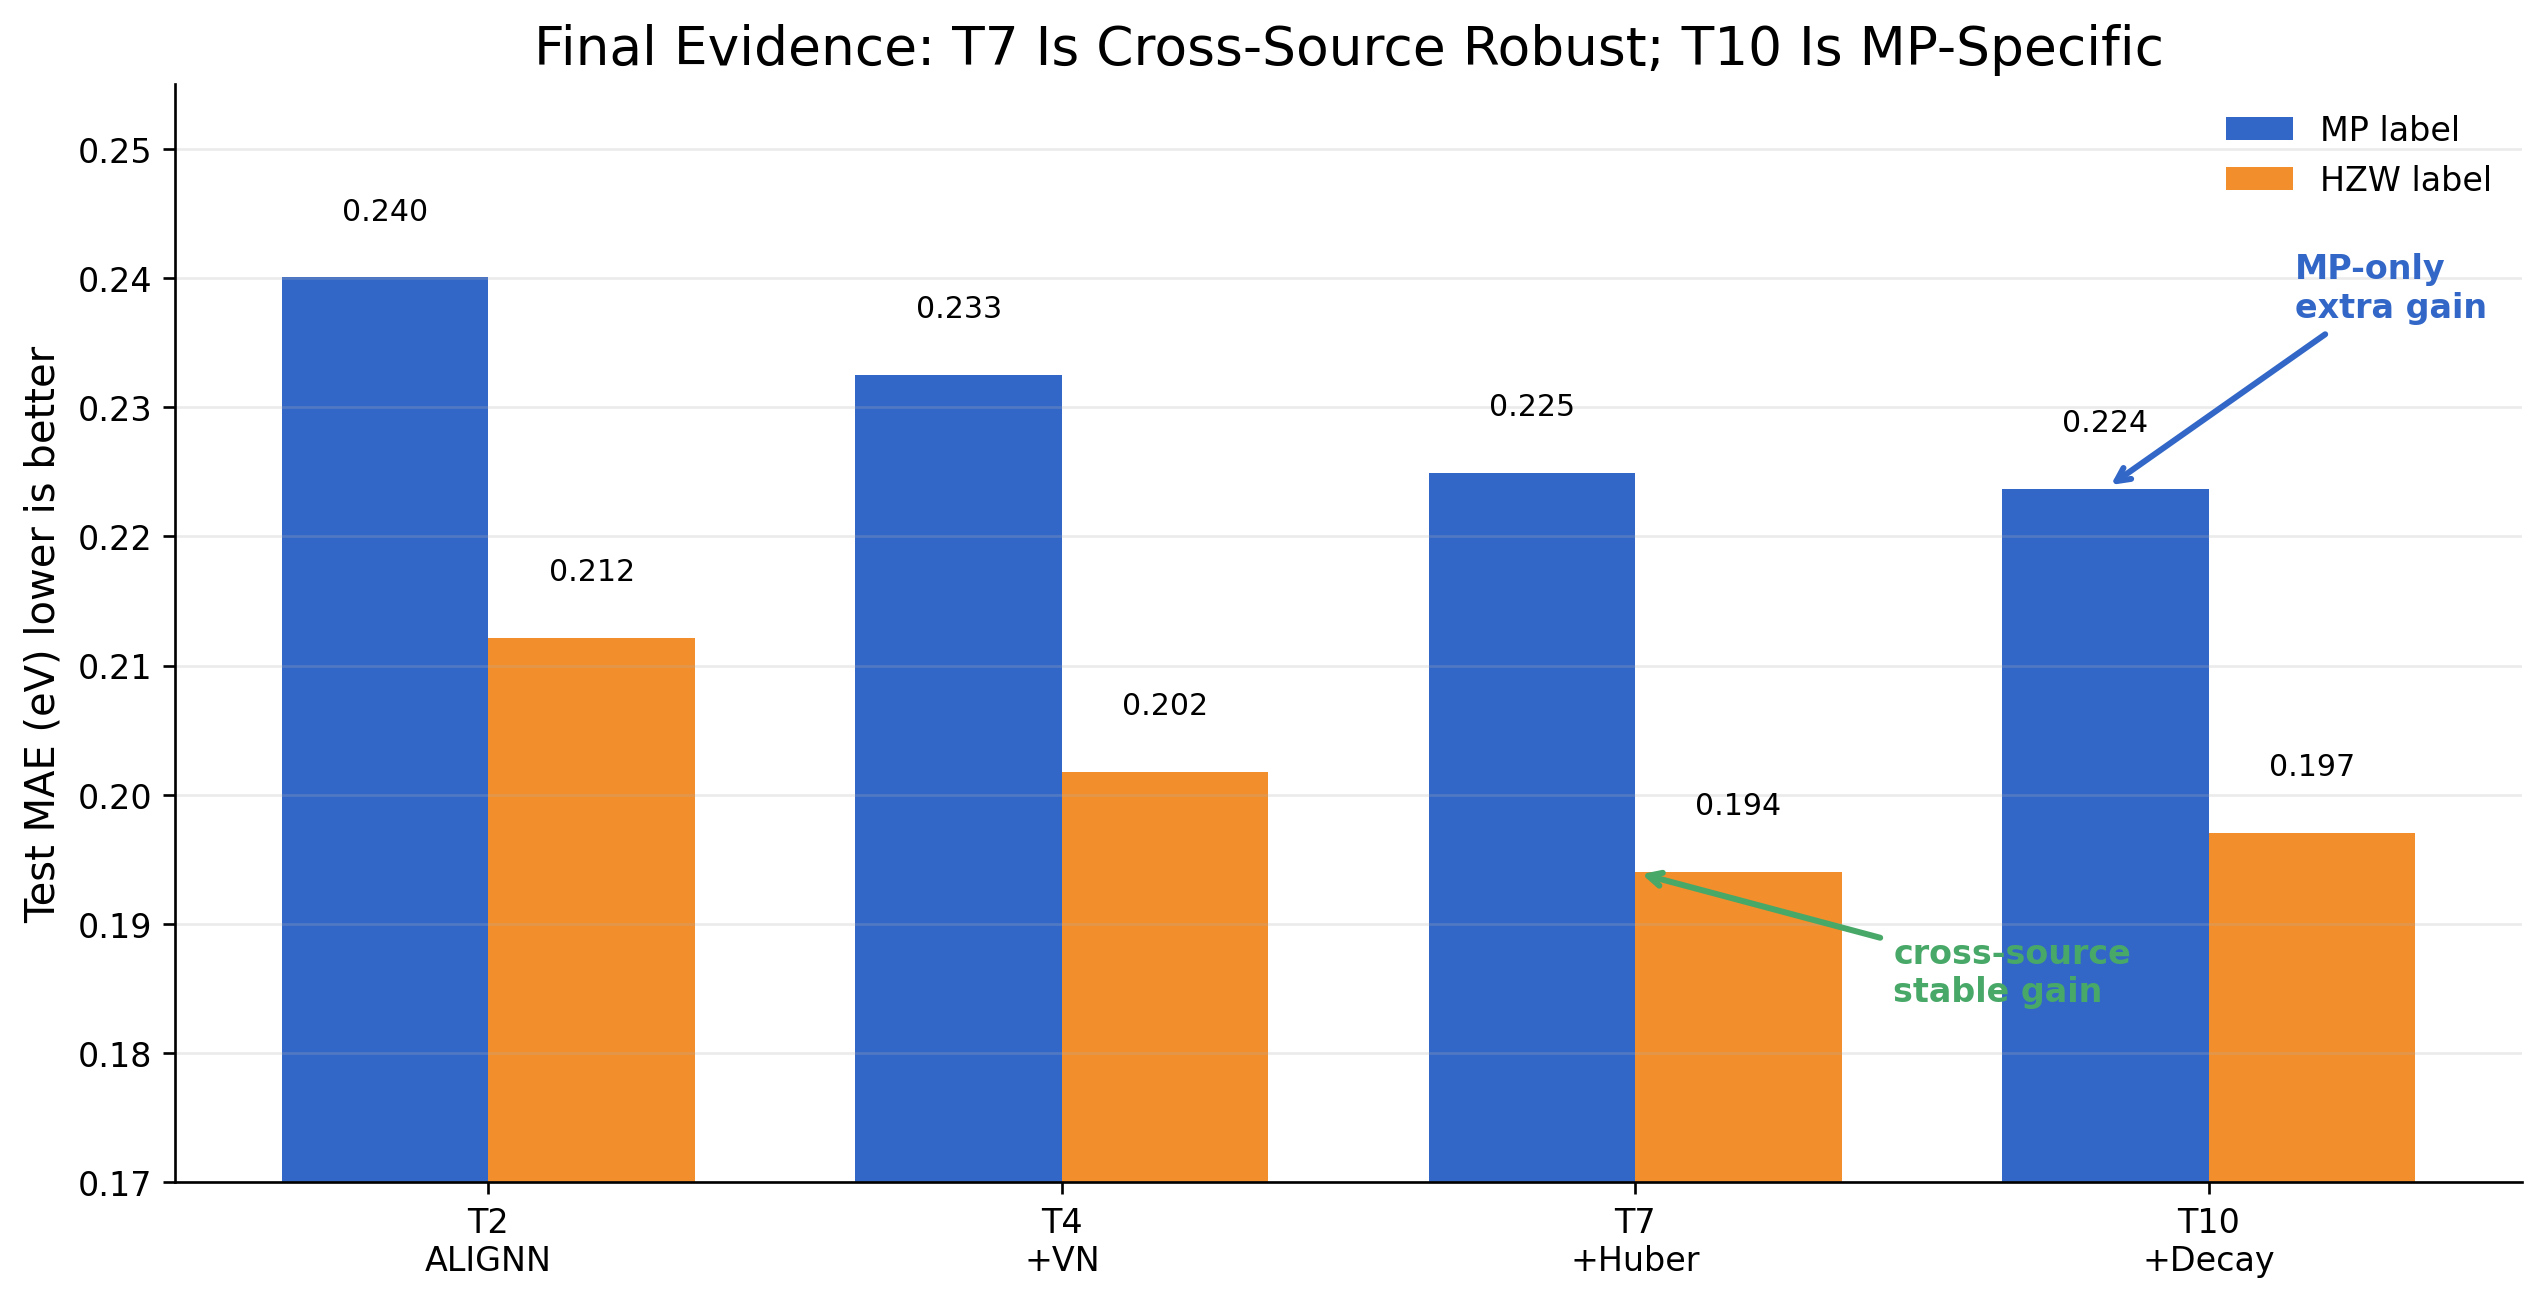
\includegraphics[width=\textwidth,height=0.76\textheight,keepaspectratio]{final_mae_bars.png}
\speakernote{这页是正文结果最适合先展示的图。讲法是：T2 到 T4 说明 single VN 有收益；T4 到 T7 说明 Huber 是跨源稳定收益；T10 在 MP 上略好，但 HZW 上回退，所以不能写成 universal best。}
\end{frame}

\begin{frame}{消融路径：真正稳定的收益来自哪里}
\centering
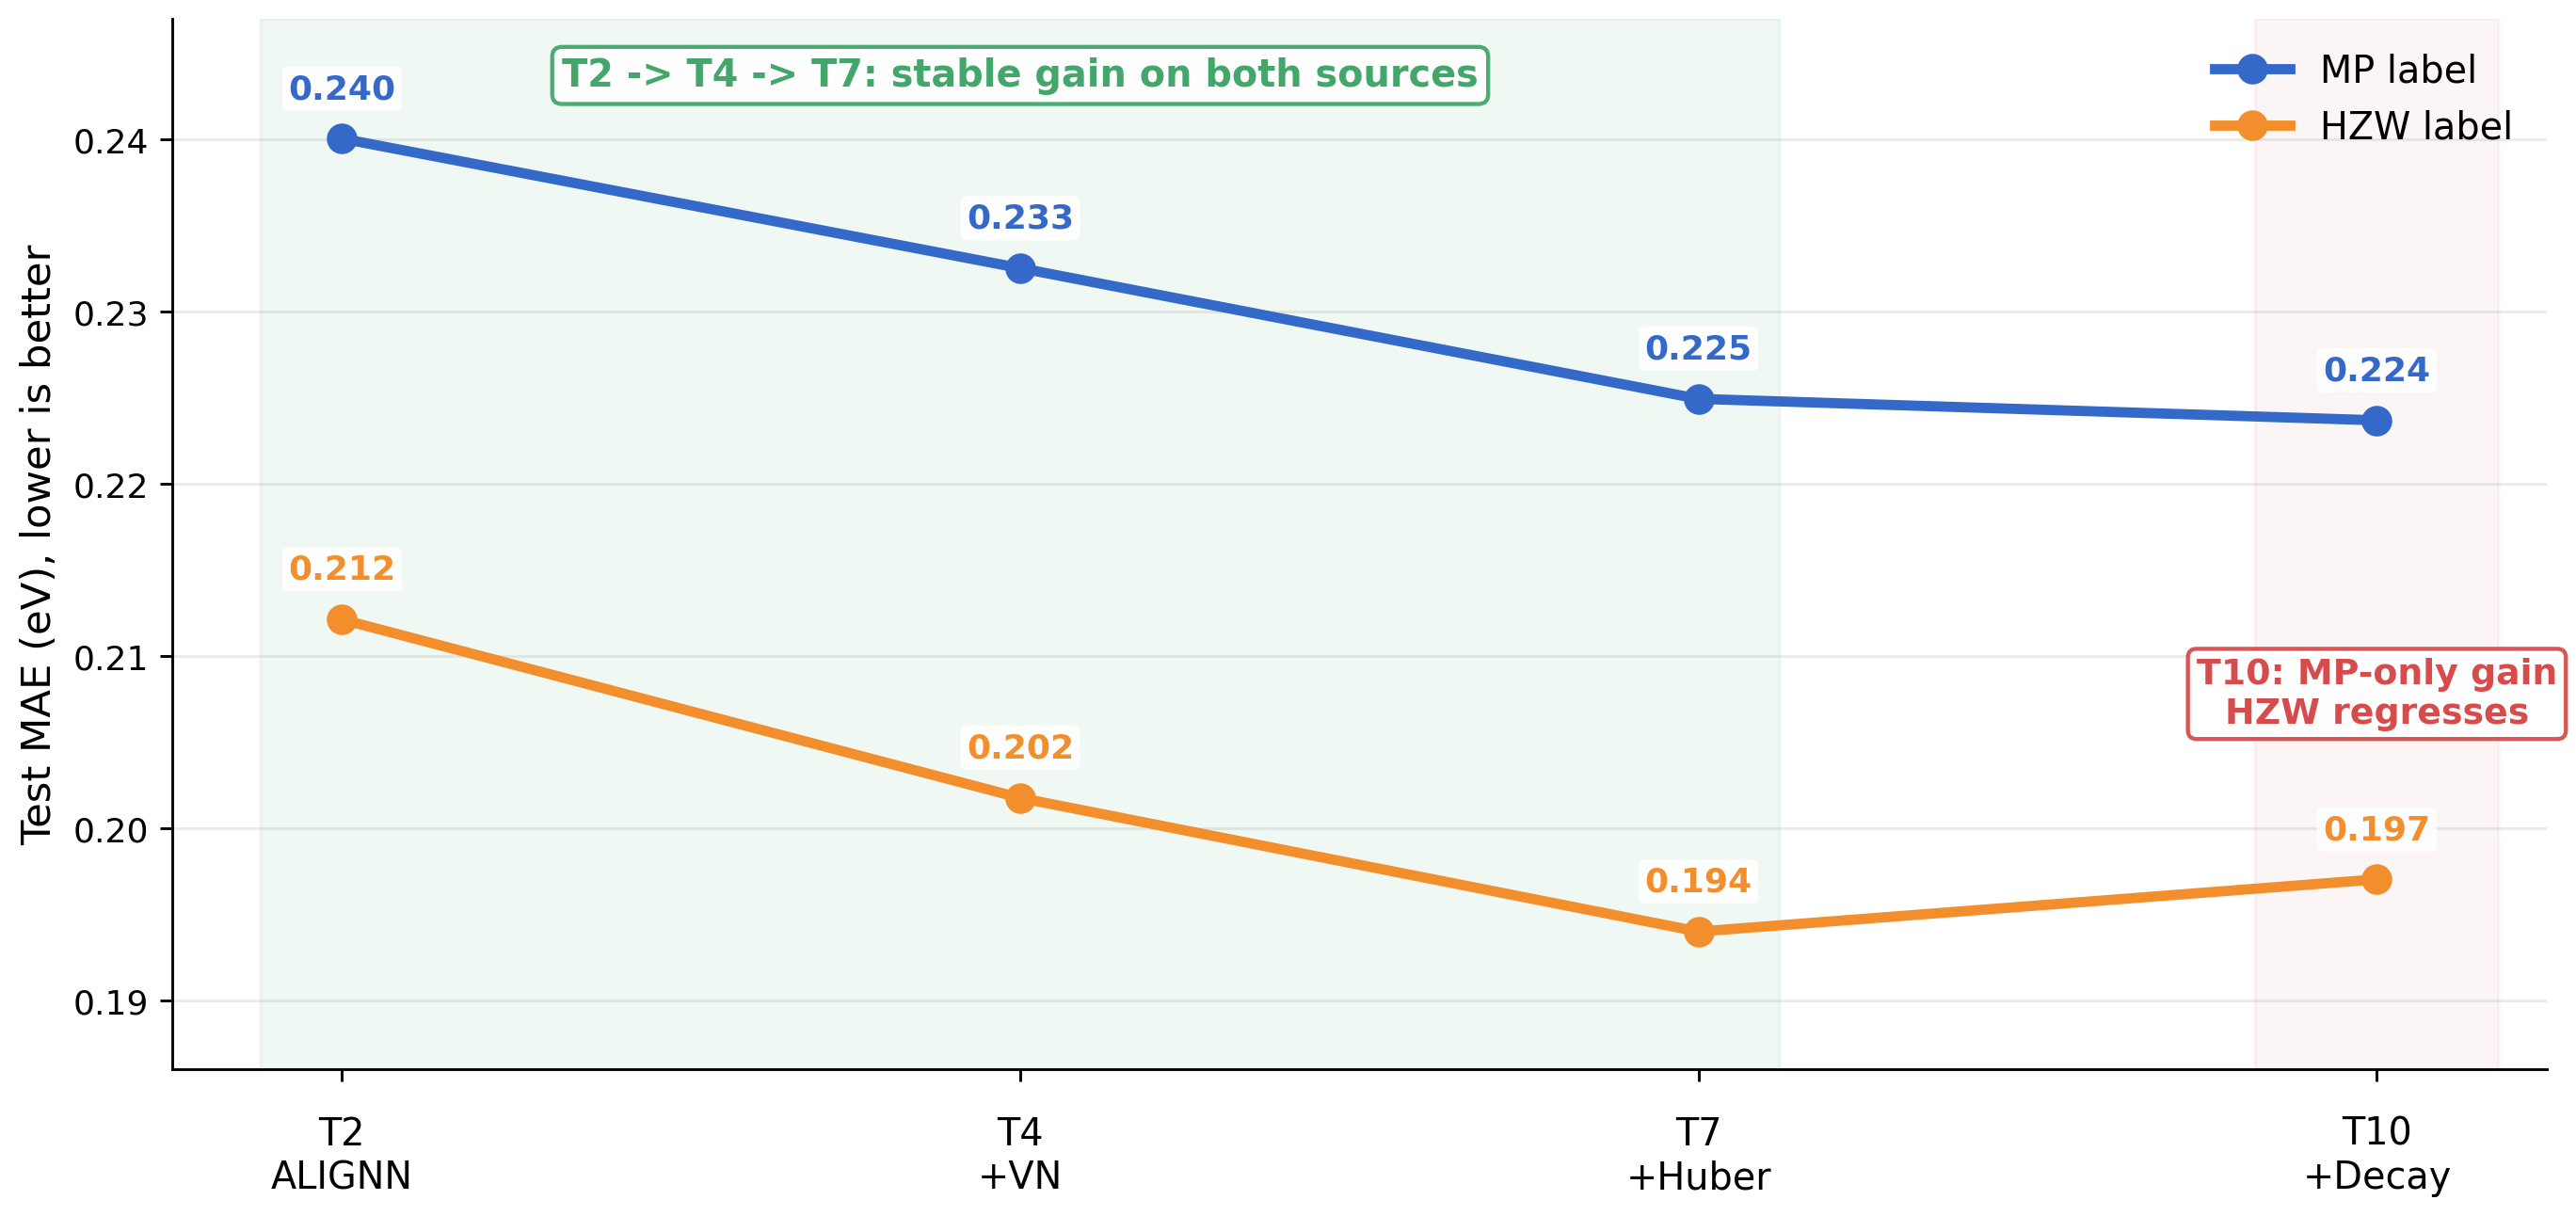
\includegraphics[width=\textwidth,height=0.76\textheight,keepaspectratio]{ablation_path.png}
\speakernote{这页帮助老师理解 T 系列不是乱做。稳定主线是 ALIGNN 到 single VN 再到 Huber；decay 是后续信息流调度，只在 MP label 有额外收益。}
\end{frame}

\begin{frame}{global token 的收益：不只看总分，也看结构分区}
\centering
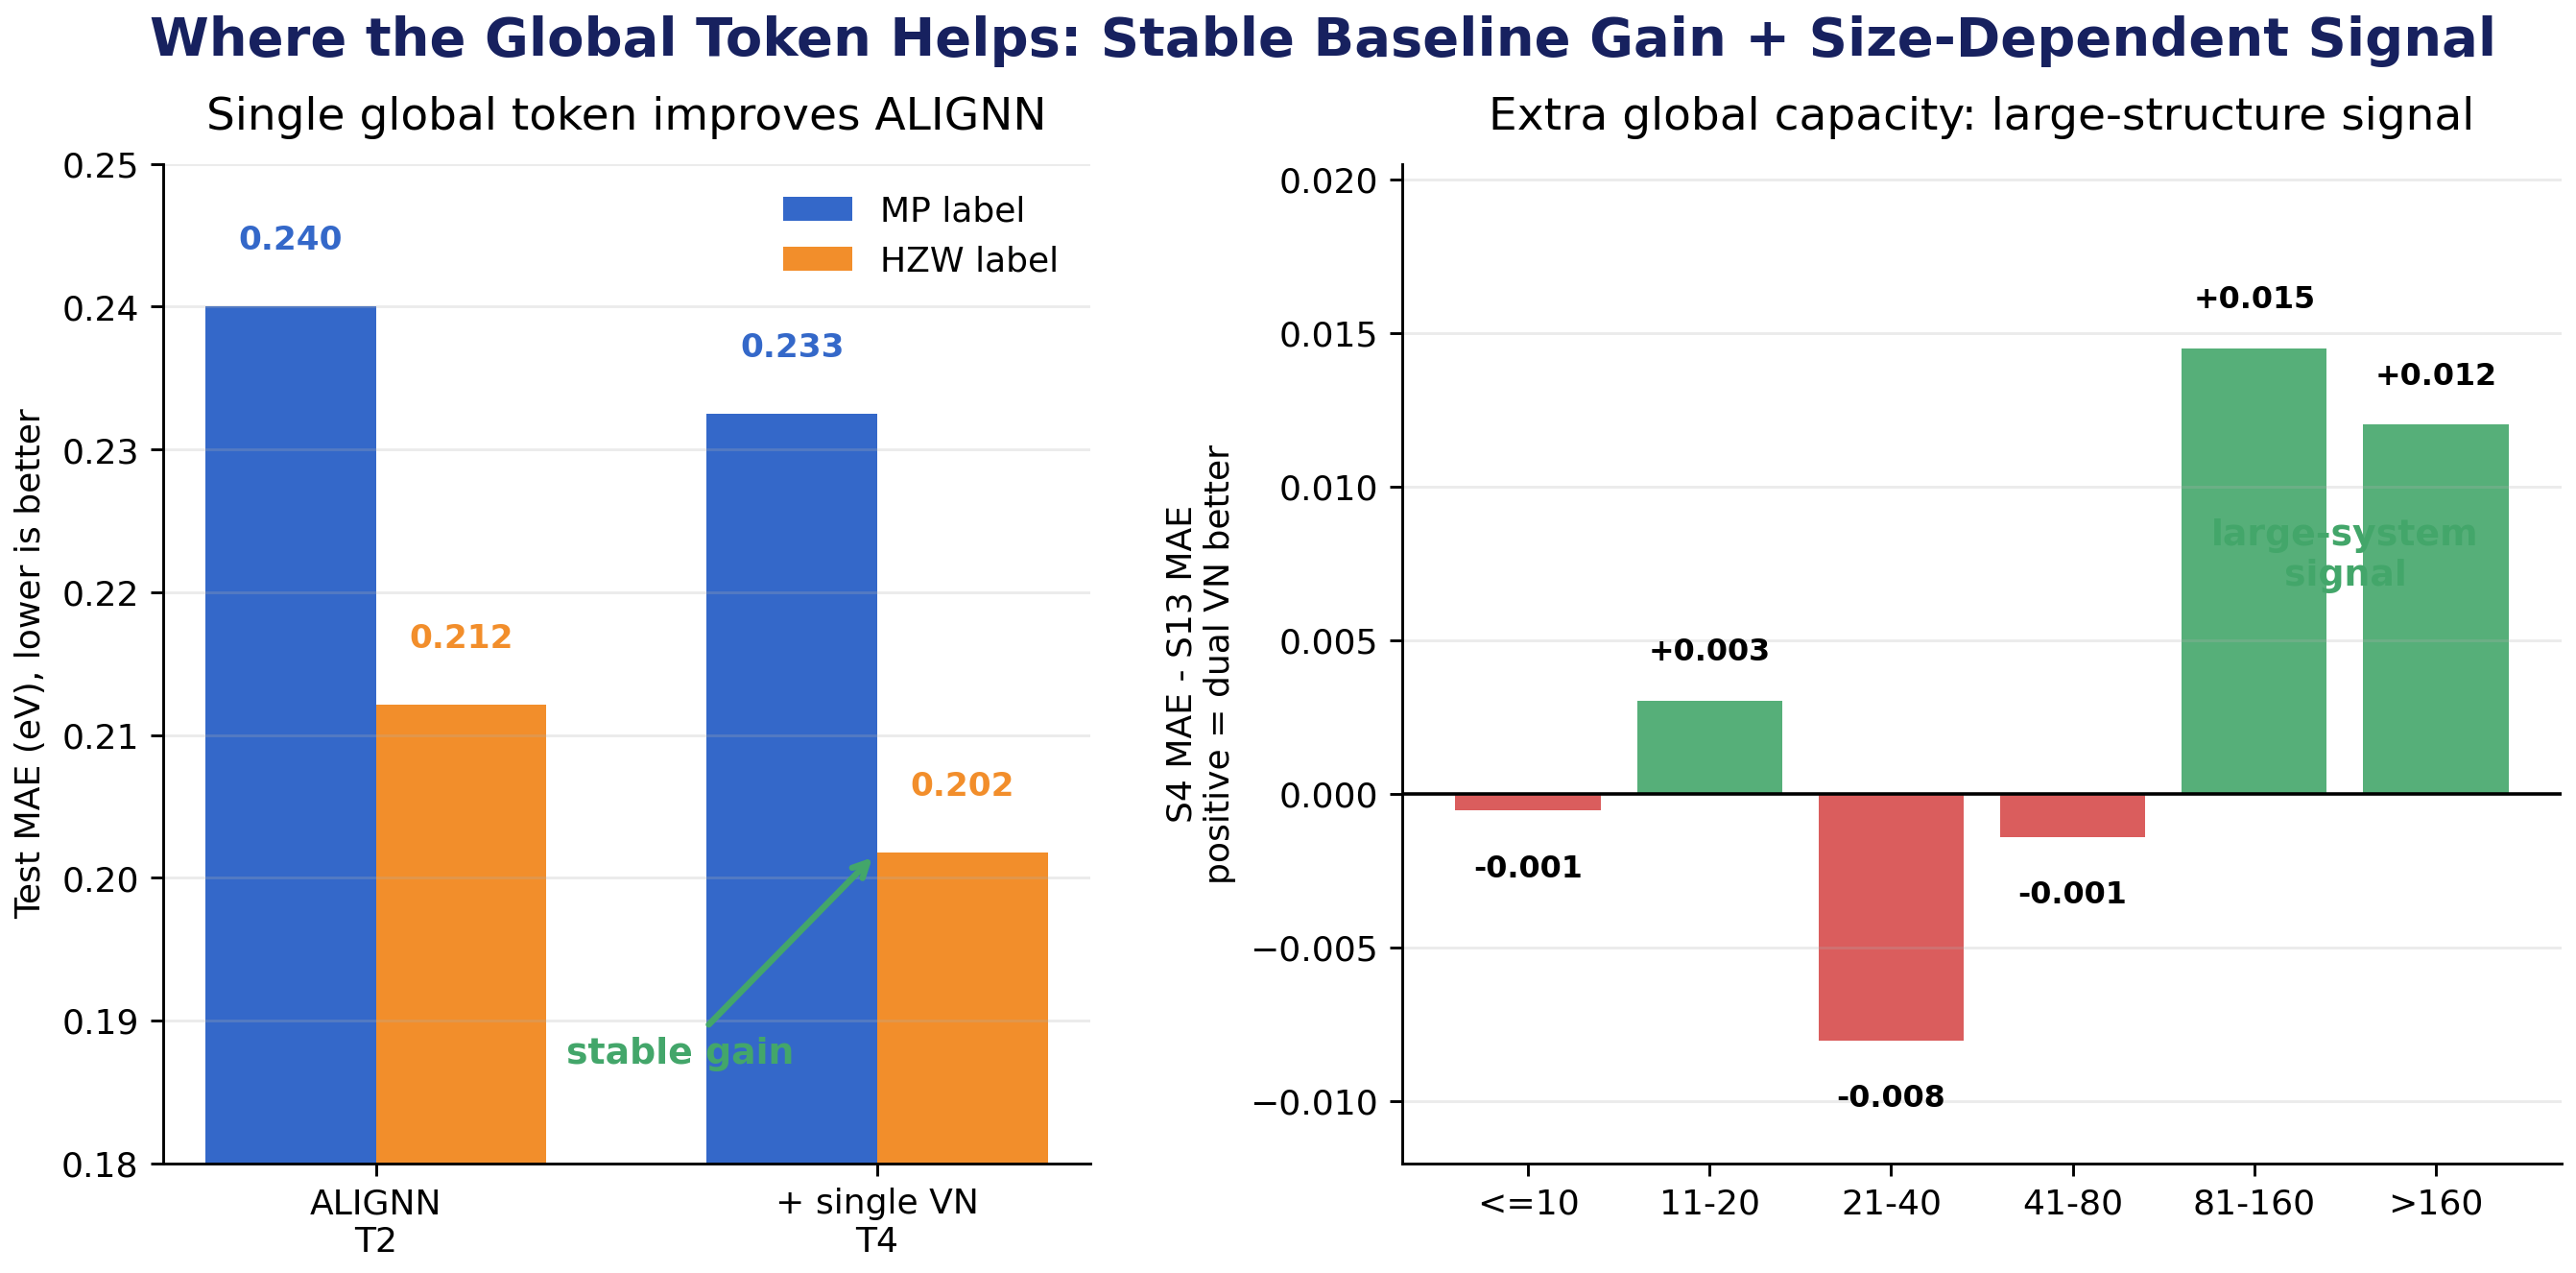
\includegraphics[width=\textwidth,height=0.76\textheight,keepaspectratio]{global_token_evidence.png}
\speakernote{这一页专门回应“global token 带来的收益怎么展示”。左边是单 global token 相对 ALIGNN 的稳定收益，MP 和 HZW 两个标签源都下降；右边是双 global token 的大小体系信号，总分不一定赢，但在 81--160 和 >160 的大结构桶里有明确正收益。论文里可以把左图放正文，右图作为 global token 对大结构更有价值的证据，细表放 SI。}
\end{frame}

\begin{frame}{Discussion 章节必须回答的问题}
\small
\begin{block}{问题 1：为什么复杂全局机制不稳定？}
Band gap 很多信息由局部化学环境和键角决定；ALIGNN 已经很强。复杂全局机制增加容量，也增加学习标签噪声的风险。
\end{block}

\begin{block}{问题 2：为什么 global decay 只在 MP 有效？}
Decay 是训练后期削弱 global-to-node 广播。MP label 受益于减少全局过校正；HZW label 反而需要持续全局校准。
\end{block}

\begin{block}{问题 3：最终推荐哪个模型？}
跨标签源最稳推荐 T7；MP label 单独最优可以报告 T10，但不能写成通用最优。
\end{block}
\speakernote{这页直接回应老师的问题，尤其是 decay 为什么在一个数据集有效另一个无效。}
\end{frame}

\section{正文证据}

\begin{frame}{主表 1：数据审计结果}
\scriptsize
\centering
\begin{tabular}{l r}
\toprule
项目 & 数量 \\
\midrule
Total rows & 95,462 \\
Structure matched rows & 92,787 \\
Structure unmatched rows & 39 \\
Missing MP records & 2,636 \\
\texttt{structure\_matched\_exact} & 92,507 \\
\texttt{structure\_matched\_supercell} & 280 \\
\bottomrule
\end{tabular}
\hspace{8mm}
\begin{tabular}{l r}
\toprule
结构匹配内部标签类型 & 数量 \\
\midrule
\texttt{no\_label\_conflict} & 85,478 \\
\texttt{mp\_metal\_hzw\_nonmetal} & 3,142 \\
\texttt{mp\_nonmetal\_hzw\_metal} & 3,046 \\
\texttt{same\_class\_gap\_diff\_gt\_1ev} & 1,121 \\
\bottomrule
\end{tabular}

\vspace{2mm}
\small
这张表建议放在 Data and Audit 章节，支撑“结构一致不等于标签一致”。
\speakernote{这张是论文数据章节的主证据。老师如果问为什么要双标签源验证，就用这张表回答。}
\end{frame}

\begin{frame}{主表 2：最终 MP label 结果}
\scriptsize
\centering
\resizebox{\textwidth}{!}{
\begin{tabular}{l l c c c c c}
\toprule
实验 & 模型 & MAE$\downarrow$ & RMSE$\downarrow$ & $R^2\uparrow$ & Metal F1$\uparrow$ & Best Epoch \\
\midrule
T1 & CGCNN & 0.366338 & 0.612696 & 0.858769 & 0.788246 & 49 \\
T2 & ALIGNN & 0.240043 & 0.490694 & 0.909414 & 0.882637 & 50 \\
T3 & M3GNet & 0.285903 & 0.584315 & 0.871550 & 0.889726 & 41 \\
T4 & single VN & 0.232520 & 0.505610 & 0.903823 & 0.909240 & 49 \\
T7 & Huber-only & 0.224931 & 0.503546 & 0.904607 & 0.911331 & 49 \\
T10 & global decay + Huber & \best{0.223686} & 0.497333 & 0.906946 & \best{0.915455} & 47 \\
\bottomrule
\end{tabular}
}

\vspace{2mm}
\small
论文写法：MP label 下 T10 最优，但 T4$\rightarrow$T7 已说明 Huber 是主收益。
\speakernote{这张表正文可以简化，只保留关键模型。完整 T1 到 T10 可以放附录或补充表。}
\end{frame}

\begin{frame}{主表 3：最终 HZW label 结果}
\scriptsize
\centering
\resizebox{\textwidth}{!}{
\begin{tabular}{l l c c c c c}
\toprule
实验 & 模型 & MAE$\downarrow$ & RMSE$\downarrow$ & $R^2\uparrow$ & Metal F1$\uparrow$ & Best Epoch \\
\midrule
T1 & CGCNN & 0.338152 & 0.565454 & 0.878497 & 0.788237 & 49 \\
T2 & ALIGNN & 0.212124 & 0.436147 & 0.927713 & 0.890299 & 50 \\
T3 & M3GNet & 0.256572 & 0.535916 & 0.890859 & 0.892629 & 43 \\
T4 & single VN & 0.201762 & 0.448621 & 0.923519 & 0.909613 & 49 \\
T7 & Huber-only & \best{0.194002} & \best{0.445837} & \best{0.924465} & 0.915401 & 49 \\
T10 & global decay + Huber & 0.197034 & 0.453592 & 0.921815 & 0.913209 & 45 \\
\bottomrule
\end{tabular}
}

\vspace{2mm}
\small
论文写法：HZW label 下 T7 最优，说明 T10 的收益不是跨源通用。
\speakernote{这张表和 MP 表必须成对出现。这样才能支撑跨数据源最稳结论是 T7，而不是 T10。}
\end{frame}

\begin{frame}{主表 4：关键消融关系}
\scriptsize
\centering
\setlength{\tabcolsep}{4pt}
\begin{tabularx}{\textwidth}{p{2.2cm} c c Y}
\toprule
对比 & MP MAE & HZW MAE & 论文解释 \\
\midrule
T2 $\rightarrow$ T4 & 0.240043 $\rightarrow$ 0.232520 & 0.212124 $\rightarrow$ 0.201762 & single VN 稳定提升 ALIGNN。 \\
T4 $\rightarrow$ T7 & 0.232520 $\rightarrow$ 0.224931 & 0.201762 $\rightarrow$ 0.194002 & Huber-only 是跨源最稳定收益。 \\
T4 $\rightarrow$ T8 & 0.232520 $\rightarrow$ 0.230402 & 0.201762 $\rightarrow$ 0.202603 & top-k-only 不是稳定贡献。 \\
T7 $\rightarrow$ T10 & 0.224931 $\rightarrow$ 0.223686 & 0.194002 $\rightarrow$ 0.197034 & decay 是 MP label 特化，不是跨源通用最优。 \\
\bottomrule
\end{tabularx}
\speakernote{这张表是 Results 和 Discussion 的连接。它把实验表转换成论文结论。}
\end{frame}

\begin{frame}{重点解释：global decay 为什么不跨源稳定}
\scriptsize
\centering
\begin{tabular}{l l c c c c}
\toprule
Dataset & Model & MAE & RMSE & Bias & P90 AE \\
\midrule
MP & T7 Huber & 0.224931 & 0.503546 & 0.025437 & 0.582403 \\
MP & T10 decay + Huber & \best{0.223686} & \best{0.497333} & \best{0.013963} & 0.588758 \\
HZW & T7 Huber & \best{0.194001} & \best{0.445837} & 0.025182 & \best{0.498598} \\
HZW & T10 decay + Huber & 0.197033 & 0.453592 & \best{0.010850} & 0.507704 \\
\bottomrule
\end{tabular}

\vspace{2mm}
\small
解释：decay 都降低了 bias，但 MP 上整体误差下降；HZW 上普通样本和高分位误差变差，说明 HZW 更依赖持续 global calibration。
\speakernote{这是老师问的重点。要讲清楚：decay 是信息流调度，不是绝对更强。它在 MP 上减少过校正，在 HZW 上削弱了有用的全局校准。}
\end{frame}

\begin{frame}{Decay 的分桶证据：不是所有结构都同向受益}
\centering
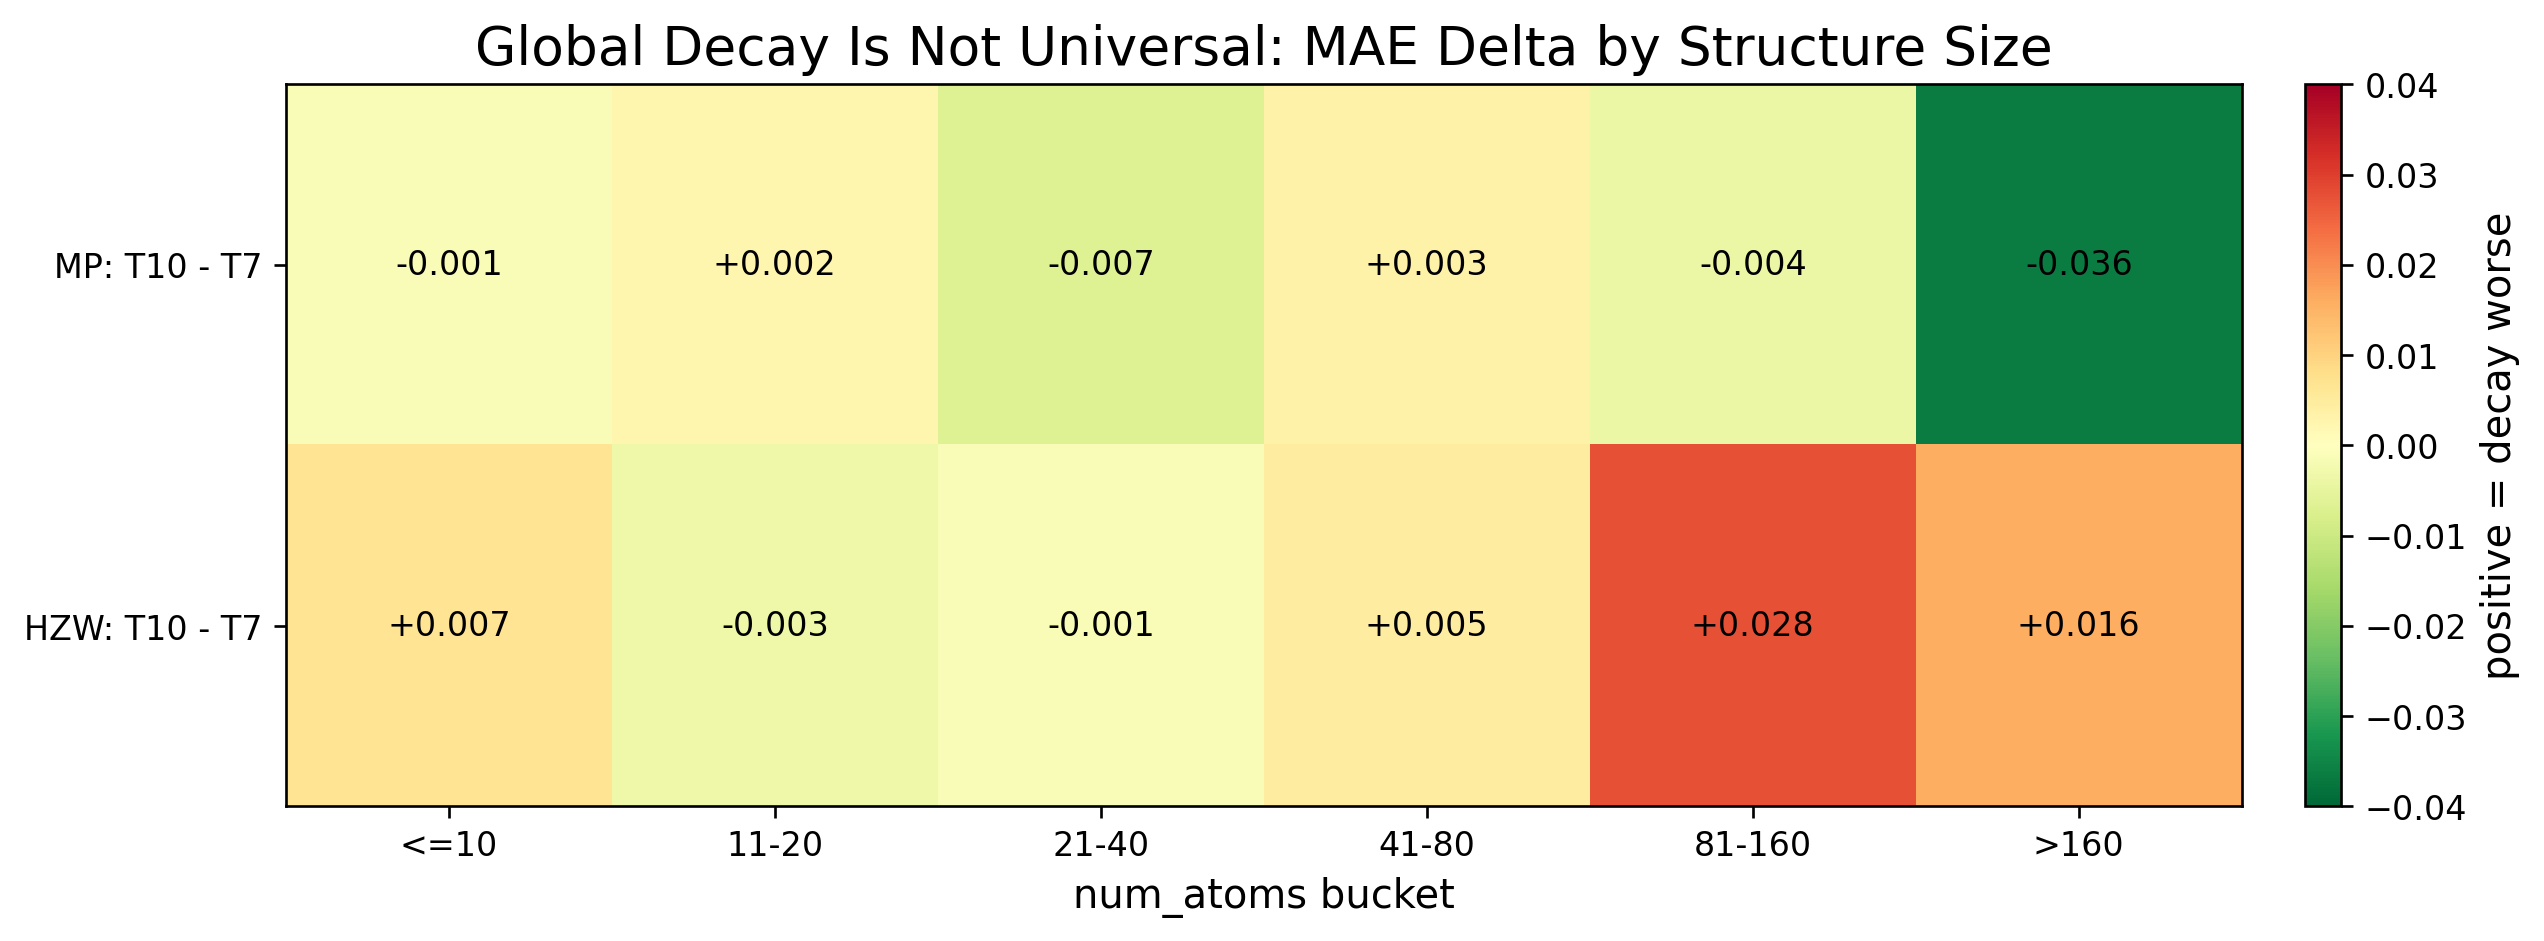
\includegraphics[width=\textwidth,height=0.75\textheight,keepaspectratio]{decay_delta_heatmap.png}
\speakernote{热力图里负数表示 T10 比 T7 好，正数表示 T10 更差。MP 在大结构尤其 >160 上受益明显；HZW 在大结构反而变差。这支撑了“decay 是 MP label 特化”的说法。}
\end{frame}

\begin{frame}{过平滑诊断：global token 的收益集中在大结构}
\centering
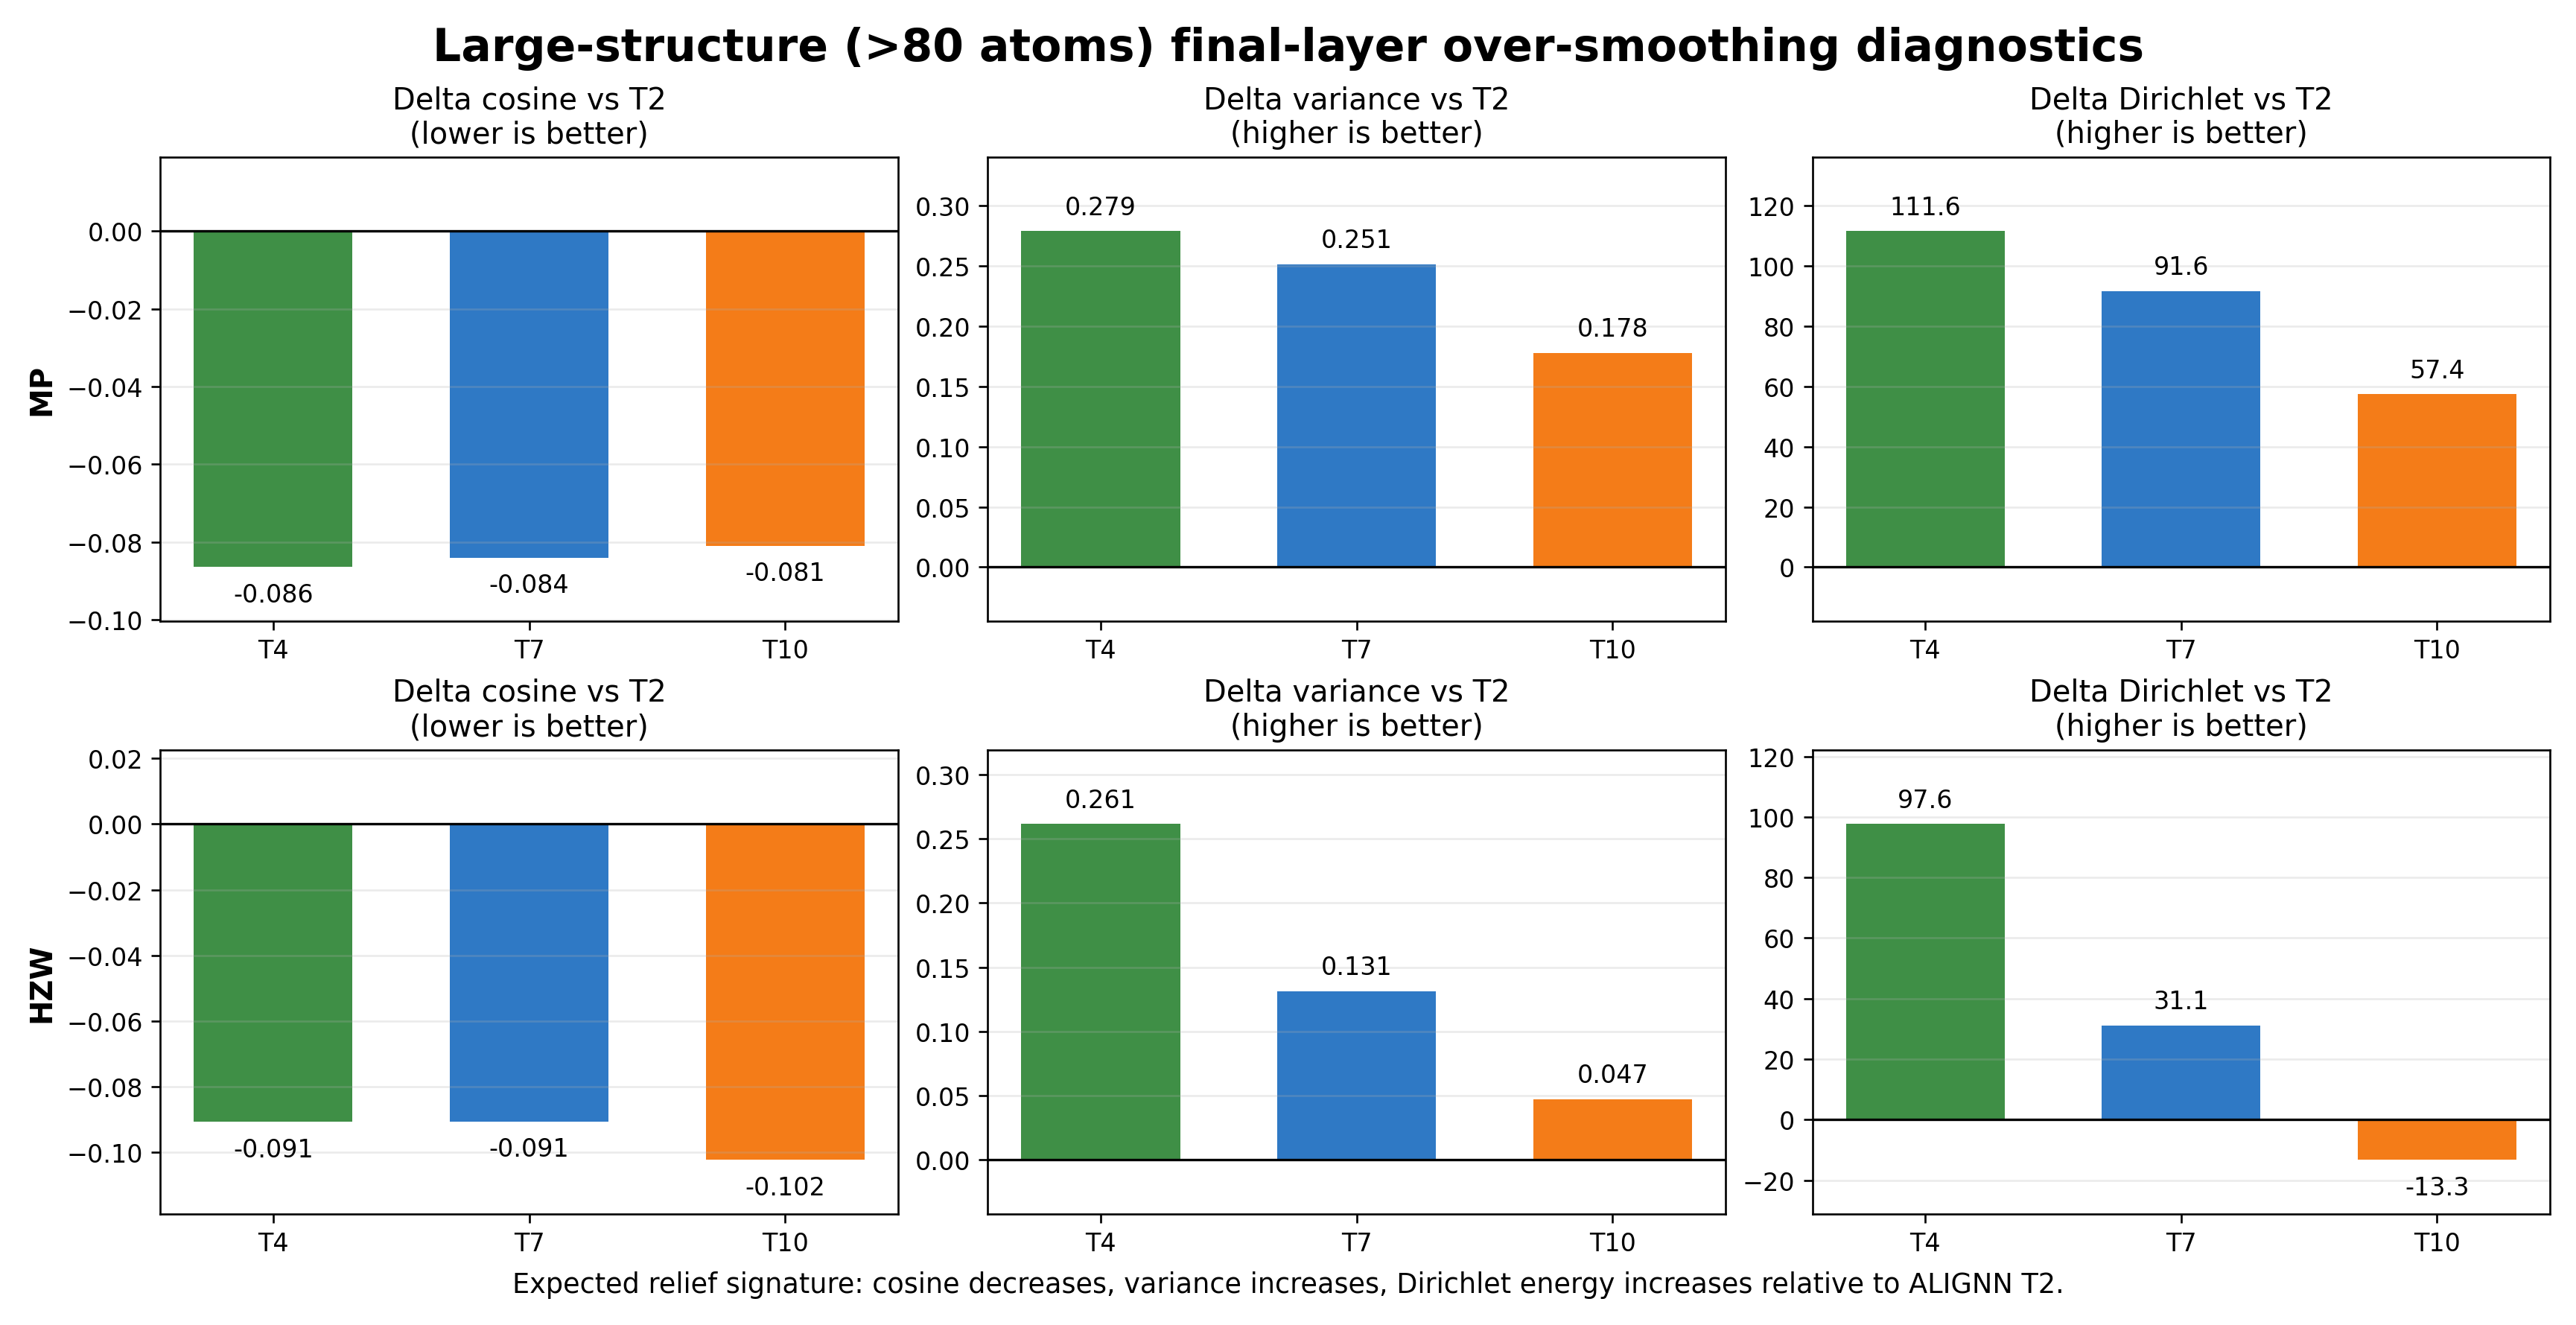
\includegraphics[width=\textwidth,height=0.75\textheight,keepaspectratio]{oversmoothing_large_structure_evidence.png}
\speakernote{这一页要谨慎讲。我们已经用 hook 抓了 T2、T4、T7、T10 的 layer-wise node embedding，但结论不是“global token 普遍解决 over-smoothing”。全样本上 cosine 不支持这个强结论；真正成立的是大结构条件结论：>80 atoms 时，T4/T7 相对 T2 的 cosine 更低、variance 更高、Dirichlet energy 更高，说明大结构上确实有缓解 embedding homogenization 的证据。}
\end{frame}

\section{图表规划}

\begin{frame}{正文和 SI 的图表分工}
\centering
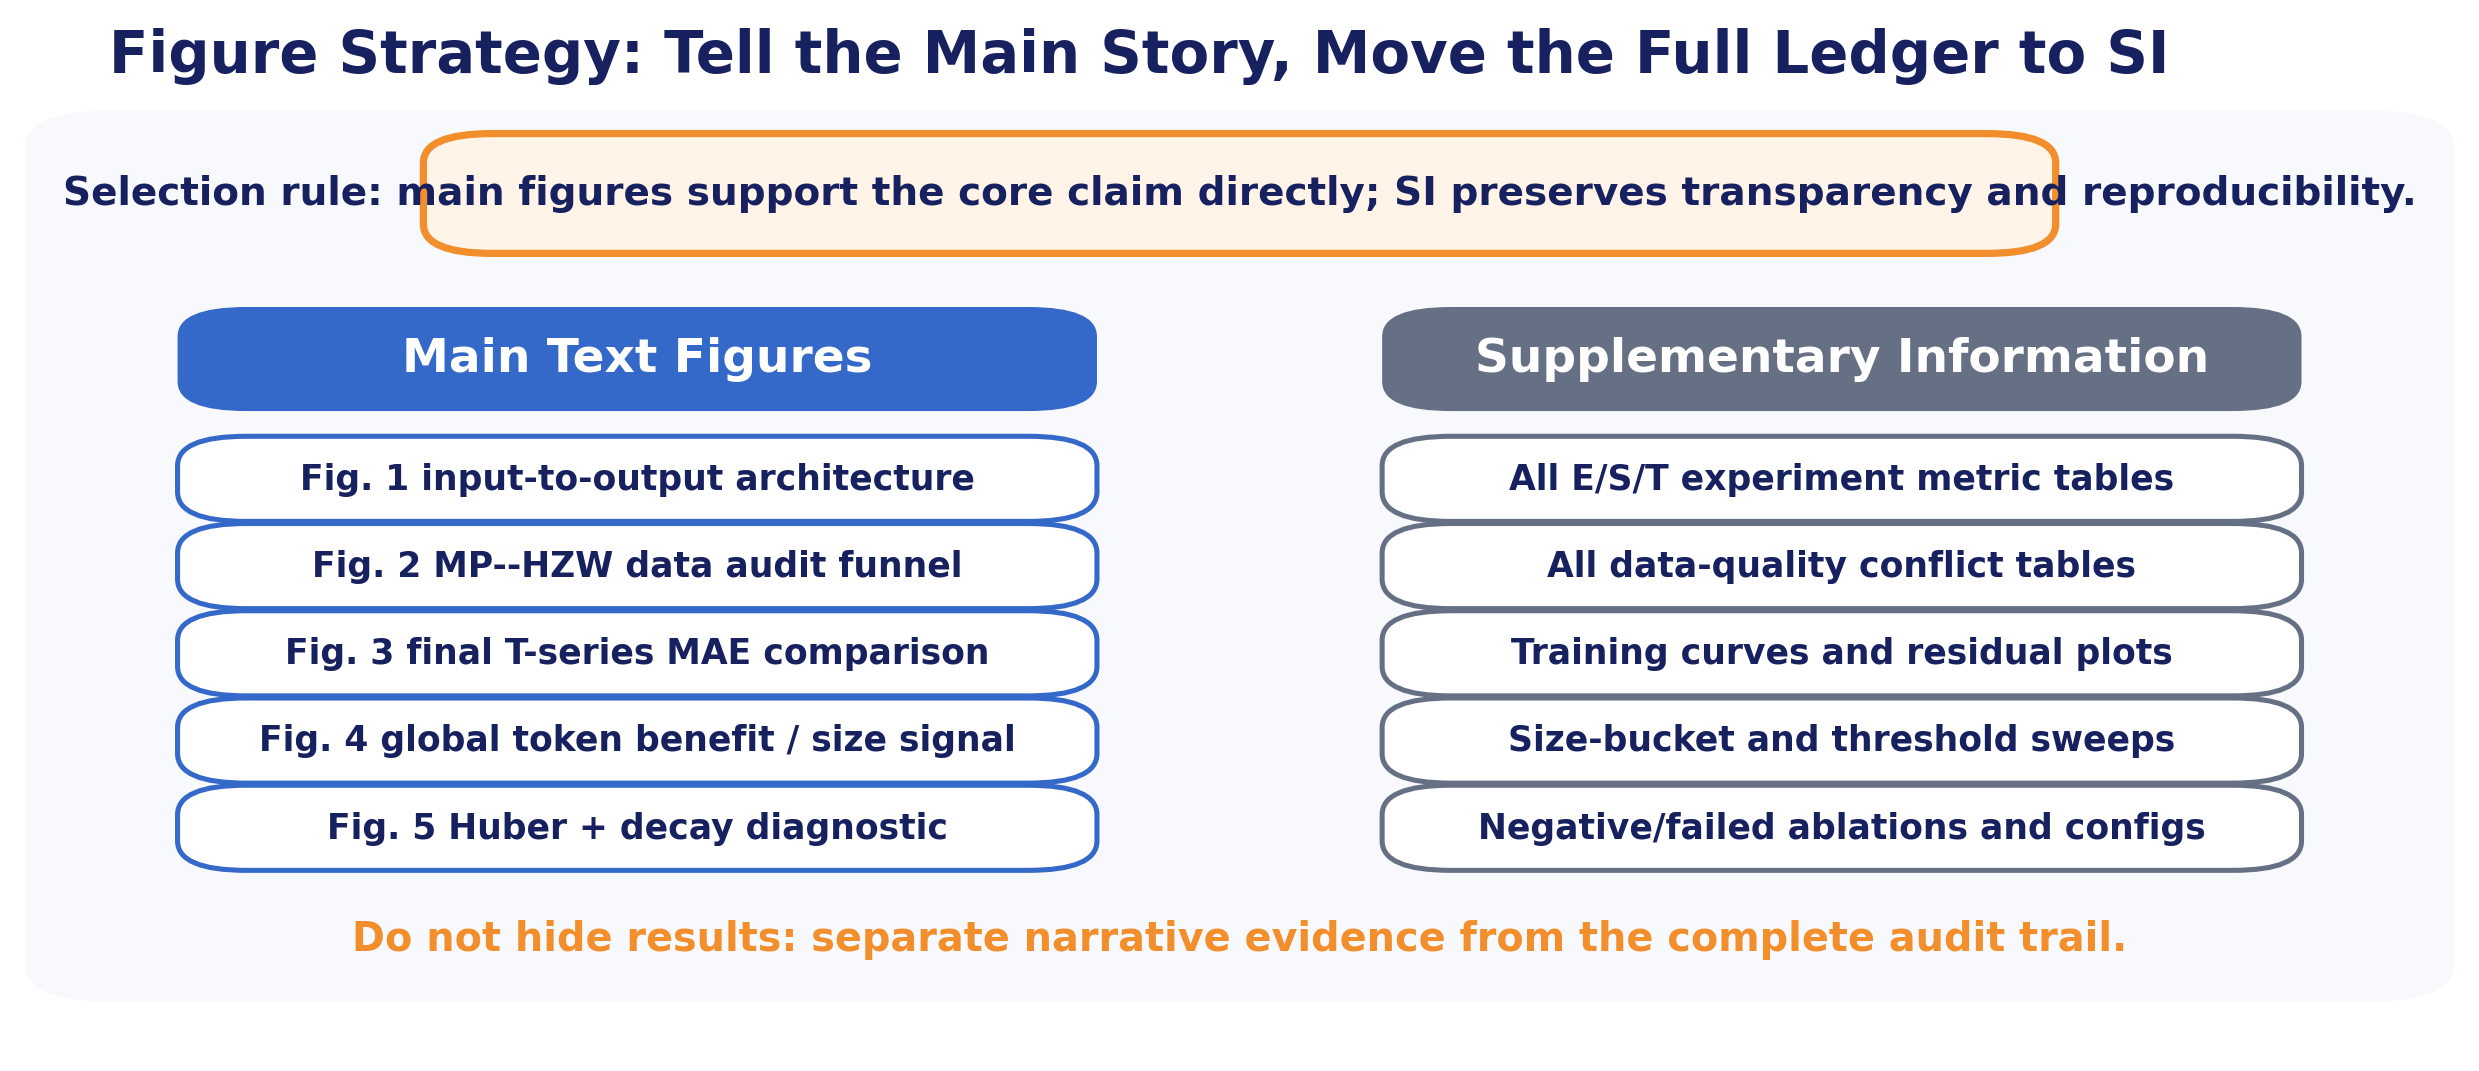
\includegraphics[width=\textwidth,height=0.76\textheight,keepaspectratio]{main_si_figure_strategy.png}
\speakernote{这页回应“所有实验和数据分析结果都可以绘制成图表，但不用全部放正文”。原则是：正文只放直接支撑论文主张的图；SI 放完整实验账本、失败消融、数据质量表、训练曲线和分桶扫描。这样既不隐藏结果，也不让正文变成流水账。}
\end{frame}

\begin{frame}{论文主图建议}
\small
\begin{tabularx}{\textwidth}{p{2.8cm} Y p{3.8cm}}
\toprule
图编号 & 内容 & 作用 \\
\midrule
Figure 1 & Input-to-output architecture：CIF/structure $\rightarrow$ graph $\rightarrow$ ALIGNN $\rightarrow$ global token $\rightarrow$ band gap。 & 补齐完整方法图。 \\
Figure 2 & MP--HZW structure-first audit funnel。 & 支撑数据贡献。 \\
Figure 3 & Final T-series MAE comparison。 & 报告主结果。 \\
Figure 4 & Global token benefit：T2$\rightarrow$T4 与大结构分桶信号。 & 体现 global token 的收益。 \\
Figure 5 & Huber / decay / over-smoothing diagnostic。 & 支撑机制讨论；过平滑只做大结构条件性结论。 \\
\bottomrule
\end{tabularx}
\speakernote{论文主图要服务故事线。input-to-output 是方法图；audit funnel 是数据图；T-series 是结果图；global token benefit 是机制图；过平滑图可以放 discussion，但只能说大结构上有条件性证据，不要写成普遍证明。}
\end{frame}

\begin{frame}{论文主表建议}
\small
\begin{tabularx}{\textwidth}{p{2.8cm} Y p{3.8cm}}
\toprule
表编号 & 内容 & 作用 \\
\midrule
Table 1 & Dataset stages and audit statistics。 & 解释数据口径。 \\
Table 2 & Model definitions：T1--T10 简表。 & 避免编号混乱。 \\
Table 3 & Final MP-label results。 & 报告 MP 上 T10 最优。 \\
Table 4 & Final HZW-label results。 & 报告 HZW 上 T7 最优。 \\
Table 5 & Ablation summary：T2/T4/T7/T8/T10。 & 提炼最终论点。 \\
Appendix A & E1--E13/E14--E21/S 系列全量索引。 & 保留探索历史，不干扰正文。 \\
\bottomrule
\end{tabularx}
\speakernote{主表要少而精。探索性实验不要全放正文，否则文章像流水账。}
\end{frame}

\begin{frame}{哪些结果进正文，哪些进附录}
\small
\begin{columns}[T,onlytextwidth]
\begin{column}{0.48\textwidth}
\begin{block}{正文}
\begin{itemize}
  \item E4/E12/E13 早期 HZW 动机。
  \item MP full 转折。
  \item MP--HZW audit 数字。
  \item 最终 T 系列 MP/HZW 双标签结果。
  \item T7/T10 decay 差异分析。
\end{itemize}
\end{block}
\end{column}
\begin{column}{0.48\textwidth}
\begin{block}{附录或补充}
\begin{itemize}
  \item E5/E7/E8 负优化细节。
  \item E14--E19 底层机制探索。
  \item E20/E21 大小体系专家。
  \item S4/S13 完整分桶表。
  \item 配置路径、训练耗时、显存。
\end{itemize}
\end{block}
\end{column}
\end{columns}
\speakernote{这一页帮助老师判断文章主线是否干净。我们保留所有探索，但不把所有探索都塞进正文。}
\end{frame}

\section{写作计划}

\begin{frame}{当前英文初稿状态}
\small
\begin{itemize}
  \item 已有英文初稿：\texttt{gnn\_bandgap\_research\_paper\_draft\_en.tex/pdf}。
  \item 已包含：Abstract、Introduction、Related Work、Data and Audit、Methods、Results、Discussion、Limitations、Conclusion、Appendix。
  \item 已写入 global decay 解释：MP 上降低过校正，HZW 上削弱有用全局校准。
  \item 当前版本更像完整技术草稿，下一步需要根据老师意见压缩/强化主线。
\end{itemize}
\speakernote{这里告诉老师不是从零开始，英文初稿已经有了。现在这份 PPT 是为了确认论文组织方式。}
\end{frame}

\begin{frame}{下一步修改优先级}
\small
\begin{enumerate}
  \item \best{先定论文主张}：T7 是跨源最稳，T10 是 MP 特化。
  \item \best{补图}：画整体 workflow、single VN 架构、data audit 流程。
  \item \best{整理主表}：把 T 系列表缩成正文主表，完整实验放附录。
  \item \best{补多 seed 或说明局限}：若时间和算力允许，优先补 T4/T7/T10 多 seed。
  \item \best{统一英文表述}：避免中文式表达和过度宣称。
\end{enumerate}
\speakernote{这页是具体工作计划。老师如果问下一步做什么，就按这个顺序回答。}
\end{frame}

\begin{frame}{最终写作边界}
\small
\begin{alertblock}{最终主张}
\centering
\best{ALIGNN + single plain virtual node + Huber loss}

是当前 MP/HZW matched band gap 任务上的跨源最稳方案。
\end{alertblock}

\begin{block}{数据源限定}
\begin{itemize}
  \item MP label 上可以报告 T10 最优。
  \item HZW label 上必须报告 T7 最优。
  \item 文章最终标题和摘要不能把 T10 写成 universal best。
\end{itemize}
\end{block}
\speakernote{结尾再次收束。最终论文要稳，不要为了看起来更强而夸大 T10。}
\end{frame}

\section{参考文献}

\begin{frame}{参考文献}
\footnotesize
\color{black}
\raggedright
\noindent [1] Tian Xie and Jeffrey C. Grossman. Crystal Graph Convolutional Neural Networks for an Accurate and Interpretable Prediction of Material Properties. \emph{Physical Review Letters}, 120(14):145301, 2018.

\vspace{0.55em}
\noindent [2] Kamal Choudhary and Brian DeCost. Atomistic Line Graph Neural Network for Improved Materials Property Predictions. \emph{npj Computational Materials}, 7:185, 2021.

\vspace{0.55em}
\noindent [3] Chi Chen and Shyue Ping Ong. A Universal Graph Deep Learning Interatomic Potential for the Periodic Table. \emph{Nature Computational Science}, 2:718--728, 2022.

\vspace{0.55em}
\noindent [4] Anubhav Jain et al. Commentary: The Materials Project: A Materials Genome Approach to Accelerating Materials Innovation. \emph{APL Materials}, 1:011002, 2013.

\vspace{0.55em}
\noindent [5] Peter J. Huber. Robust Estimation of a Location Parameter. \emph{The Annals of Mathematical Statistics}, 35(1):73--101, 1964.
\speakernote{参考文献保留核心五篇：CGCNN、ALIGNN、M3GNet、MP、Huber。Matbench 可在论文正文参考文献里保留。}
\end{frame}

\appendix
\section{Backup}

\begin{frame}{Backup：完整 T 系列定义}
\tiny
\centering
\setlength{\tabcolsep}{3pt}
\begin{tabularx}{\textwidth}{p{0.7cm} p{3.2cm} Y}
\toprule
编号 & 模型 & 变更点 \\
\midrule
T1 & CGCNN baseline & 基础晶体图卷积。 \\
T2 & ALIGNN baseline & 最强传统 baseline。 \\
T3 & M3GNet baseline & 材料图 baseline。 \\
T4 & ALIGNN + single plain VN & 稳定全局超节点。 \\
T5 & ALIGNN + plain dual VN & 双朴素超节点；最终 HZW 指标不完整。 \\
T6 & top-k VN + Huber & 稀疏 node-to-global + 鲁棒损失。 \\
T7 & single plain VN + Huber & Huber-only 消融，跨源最稳。 \\
T8 & top-k VN + MSE & top-k-only 消融。 \\
T9 & warmup top-k + Huber & 先均值汇聚，再逐渐转 top-k。 \\
T10 & decay VN + Huber & 后期降低 global-to-node 广播，MP label 最优。 \\
\bottomrule
\end{tabularx}
\speakernote{如果老师问编号细节，用这页回答。}
\end{frame}

\begin{frame}{Backup：后续可补实验}
\small
\begin{itemize}
  \item T4/T7/T10 做 3 个 seed，给出 mean $\pm$ std。
  \item 单独分析 MP--HZW 标签差异大的样本，验证 Huber 是否主要降低异常样本影响。
  \item 对 T10 decay schedule 做轻量消融：min scale 0.25/0.5/0.75。
  \item 若转任务，优先考虑介电、压电、声子等全局响应更强的性质。
\end{itemize}
\speakernote{这页是备选后续工作，不作为当前论文必须完成项。}
\end{frame}

\end{document}
